%
% $Id: blank.tex,v 2.0 2010-01-05 18:50:50+09 kobayasi Exp $
%
% Mar 21, 2001:  Revision Control Started!!
%
\documentclass[11pt]{jreport}
\usepackage{newcent}             % PDFへの変換後の品質を高める
\usepackage[dvipdfmx]{graphicx}
\usepackage{color}
\definecolor{purple}{rgb}{0.6,0,0.4}
\definecolor{brown}{cmyk}{0,0.81,1,0.60}
\usepackage{listings, jlisting}
\renewcommand{\lstlistingname}{ソース}
\lstset
{
breaklines = true,
language=Java,
keywordstyle={\color{purple}},
commentstyle={\color{brown}},
numbers=left,
frame=single,
tabsize=4
}

\renewcommand{\slash}{"/"}

%
%\usepackage[doctor]{gaiyo}      % 博士論文要旨の場合
%\usepackage[master]{gaiyo}      % 修士論文要旨の場合
\usepackage{sotsuron}               % 卒業研究概要の場合
% \usepackage[junior]{gaiyo}      % 専門演習レポートの場合

\setlength\textfloatsep{0pt}

\title{\bfseries スマートフォンのモーションセンサを利用した\\個人認証アプリケーションの開発}
\author{情11-0170 高坂 賢佑}
\date{}
\renewcommand{\bibname}{参考文献,参考URL等}

\begin{document}
\maketitle

\tableofcontents
\listoffigures

\chapter*{はじめに}
スマートフォンが徐々に普及しつつある現在,スマートフォンの個人認証方法は画面上に表示されるソフトウェアキーボードのテンキーを用いたパスコード認証が大部分を占めている.
しかし,この認証方法は画面ロックを解除するたびに画面に表示されたソフトウェアキーボードを目で見て指でタッチして操作する必要が有るため,ユーザにとって煩雑な作業である.
また,パスコード認証では,あらかじめ決められた文字種の中から1つずつ選択したものを元にパスコードを構築していくという性質上,パターン数が限られ,自由度が限定されてしまう.
そこで,パスコード認証が抱える認証の煩雑さを解消し,かつ,自由度が高くより直感的に個人認証を行えるアプリケーションを開発する.
このアプリケーションには,一般的なスマートフォンに搭載されている加速度センサとジャイロセンサを用いることとする.

\chapter{使用するセンサについて}
	\section{加速度センサ}
	加速度センサとは,X軸,Y軸,Z軸の基準軸に対して直線運動の加速度をそれぞれ検出し,値として取り出すことのできるセンサである.
	ここでいう加速度とは,端末における,単位時間あたりの速度の変化率のことを指し,図\ref{sensor}における直線で示した矢印の方向が正の値,逆が負の値をとる.
	
	\section{ジャイロセンサ}
	ジャイロセンサとは,X軸,Y軸,Z軸の基準軸に対して回転運動の角速度をそれぞれ検出し,値として取り出すことのできるセンサである.
    ここでいう角速度とは,端末における,単位時間あたりの回転角のことを指し,図\ref{sensor}における橙色で示した回転の方向が正の値,逆が負の値をとる.

    % センサのイメージ図
    \begin{figure}[htbp]
      \begin{center}
        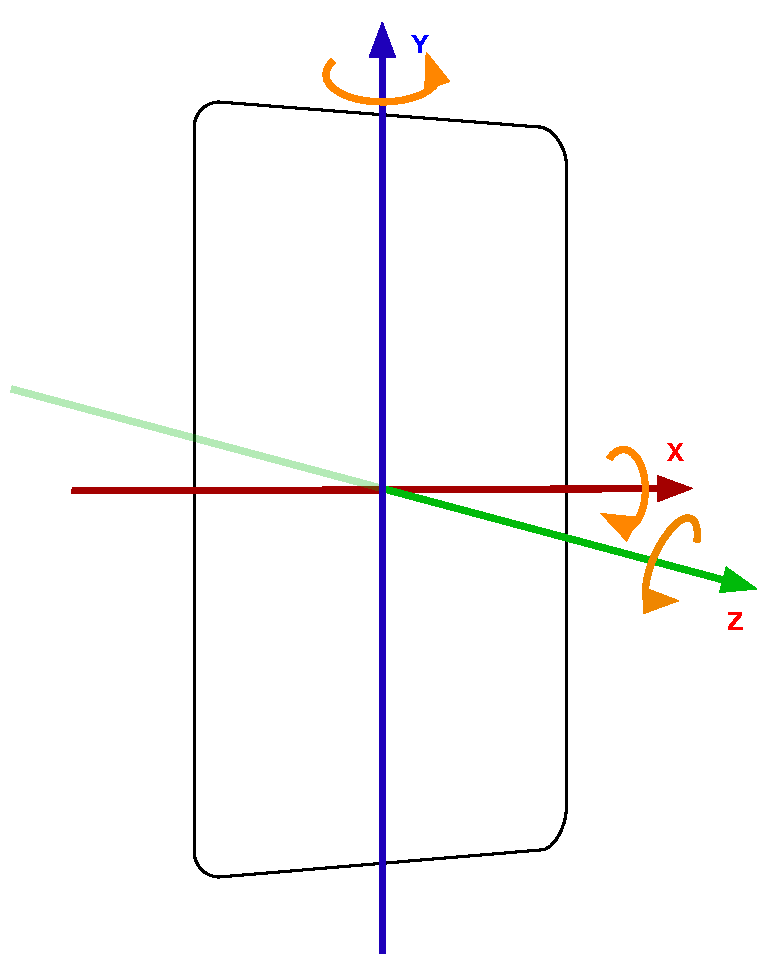
\includegraphics[width=7cm, bb=0 0 373 469]{SmartphoneSensor.pdf}
        \caption{モーションセンサの座標系イメージ}
        \label{sensor}
      \end{center}
    \end{figure}

\chapter{先行研究}
	\section{坂本の研究}
	坂本の研究では,ユーザが入力したモーションの数値化に加速度センサを用い,あらかじめ保存しておいた複数のジェスチャパターンのデータと認証時に入力したデータをパターンマッチング方式のアルゴリズムを用いて比較することで個人認証を行った.

    しかし,このプログラムは扱うジェスチャによって認証率が高いものと低いものの二分化の傾向が見られるという問題点があった.

	\section{兎澤の研究}
    兎澤の研究では,モーションの数値化に加速度センサとジャイロセンサを用い,認証システムの中核に相関関数を用いたシステムを開発し,ユーザに三回入力させたモーションの平均値データと認証時に入力したデータの類似性を調べることで個人認証を行った.
    これにより,坂本の研究で指摘されていた成功率の二分化や,立体的な動きへの対応を可能にし,モーションの対応幅を広げることができた.

    しかし,全体的な認証成功率が低く,特に手首のスナップを用いるような動きの小さいモーションに対して認証率が特に低く出るなど,対応できるモーションに限りがあるという問題点が指摘されていた.

\chapter{本研究のシステム}
	\section{本研究の概要}
	本研究では,兎澤の研究で挙げられていた,全体的な認証成功率の低さや対応できるモーションに限りがあるという点を改善することを目標とする.
    具体的には,より幅広いモーション,特に手首のスナップを用いるような比較的動きの小さいモーションに対しての,個人認証の全体的な認証成功率の向上を目指し,より実用レベルに近いアプリケーションの開発を行う.

	\section{システムの概要}
	本研究では,先行研究をもとにAndroidデバイス上で動作するアプリケーションとしてシステムを構築する.
    システムの動作フローを図\ref{flow}に示す.

    % システム動作フロー図
    \begin{figure}[htbp]
        \begin{center}
            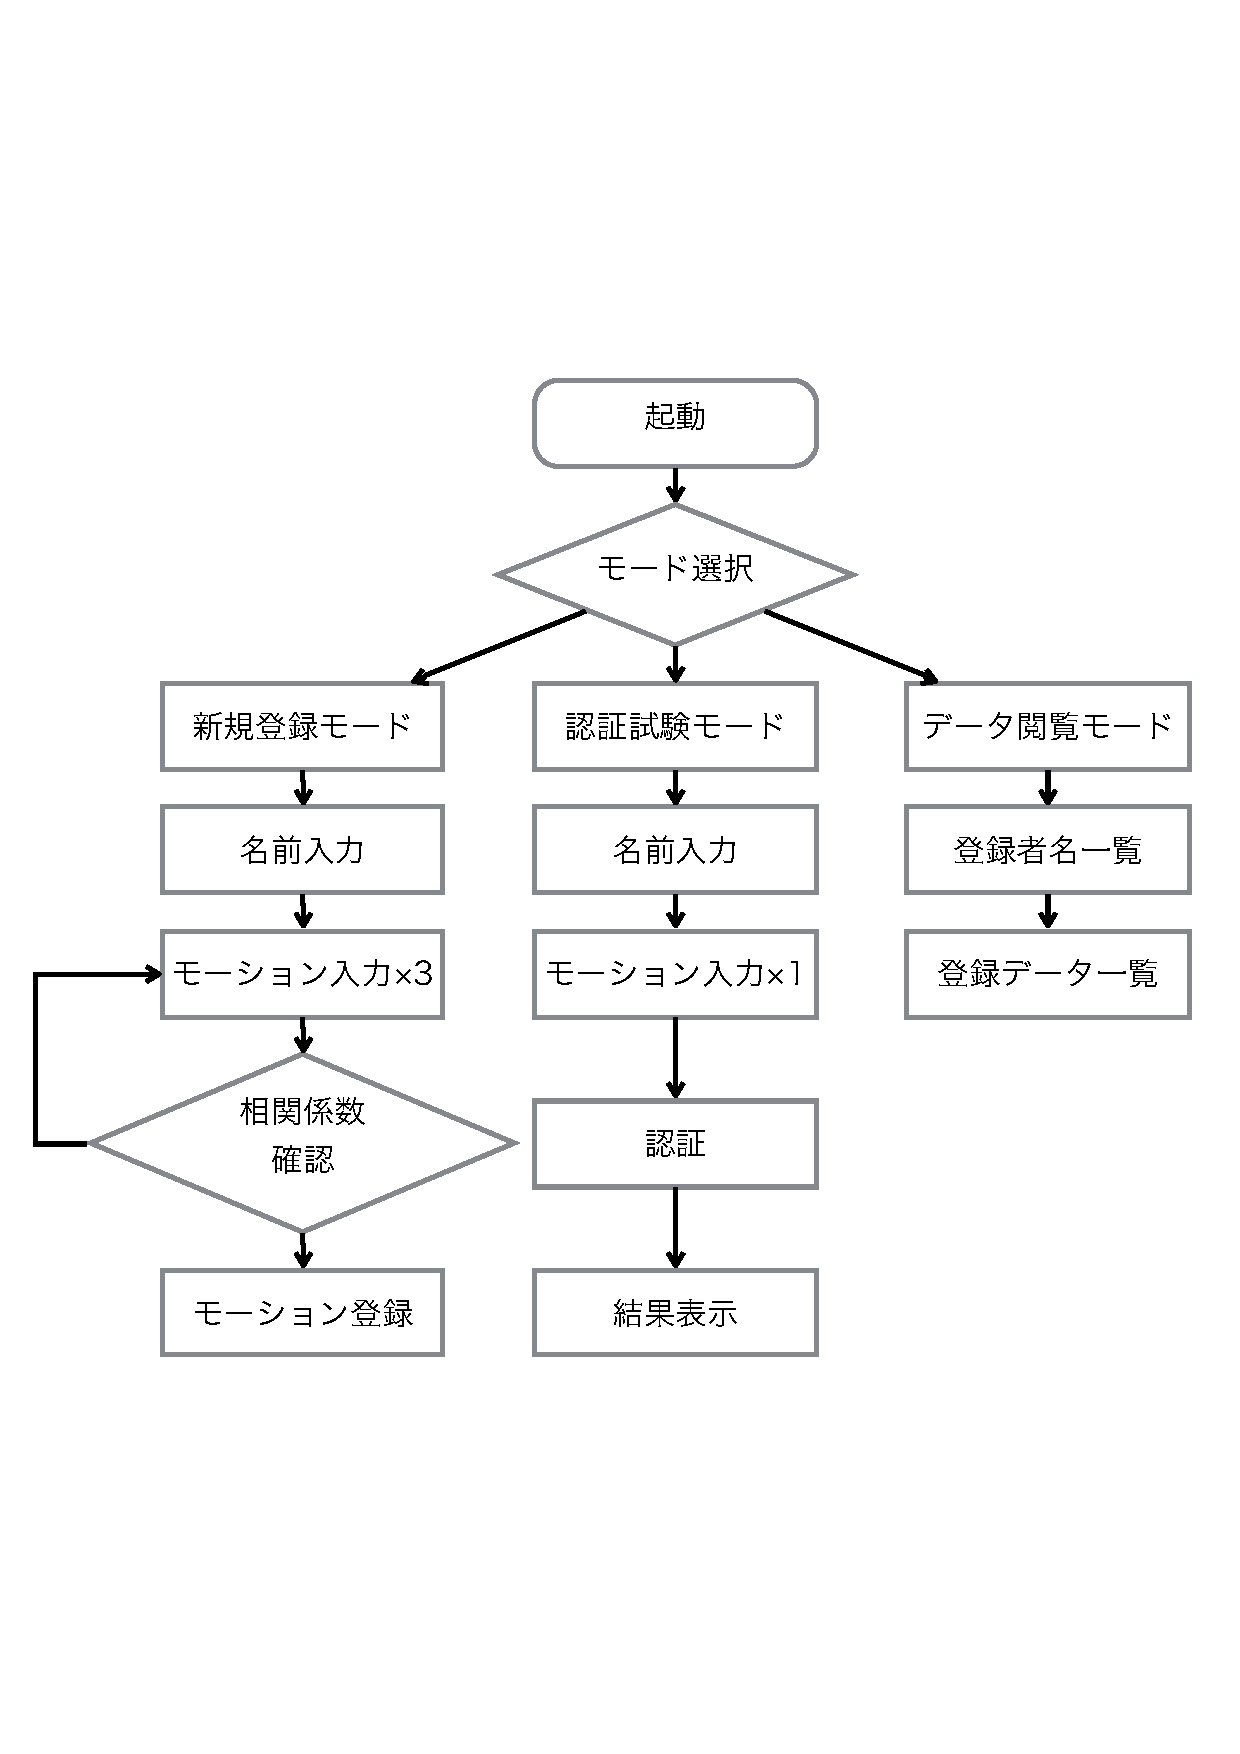
\includegraphics[width=7cm, bb=0 183 594 670]{Flow.pdf}
            \caption{システム動作フロー図}
            \label{flow}
        \end{center}
    \end{figure}

    アプリケーション起動時は,図\ref{start}のような起動画面が表示される.
    ここでStartボタンを押すことで,図\ref{selectMode}のようなモード選択ダイアログが表示される.

    ユーザはまず,新規登録モードにおいて個人認証に用いる鍵情報となるモーションを登録する.
    新規登録モードでは,ユーザに同一のモーションを三回入力させ,入力した三回のモーションが同一のモーションであると確認できた場合にそのモーションの平均値をユーザのモーションデータとして登録する.

    個人認証時には,事前に新規登録モードにおいてモーションデータを登録しておいたユーザ名を入力させ,該当ユーザが登録されていると確認できた場合にのみ,ユーザにモーションを一回入力させる.
    入力されたモーションデータと指定したユーザ名で登録されたモーションデータ間の相関を取ることで個人認証を行う.

    また,新規登録モードにおいて登録したユーザ名および登録データに関しては,データ閲覧モードにおいて閲覧することが可能である.

    % スタート画面スクリーンショット
    \begin{figure}[htbp]
        \begin{minipage}{0.5\hsize}
            \begin{center}
                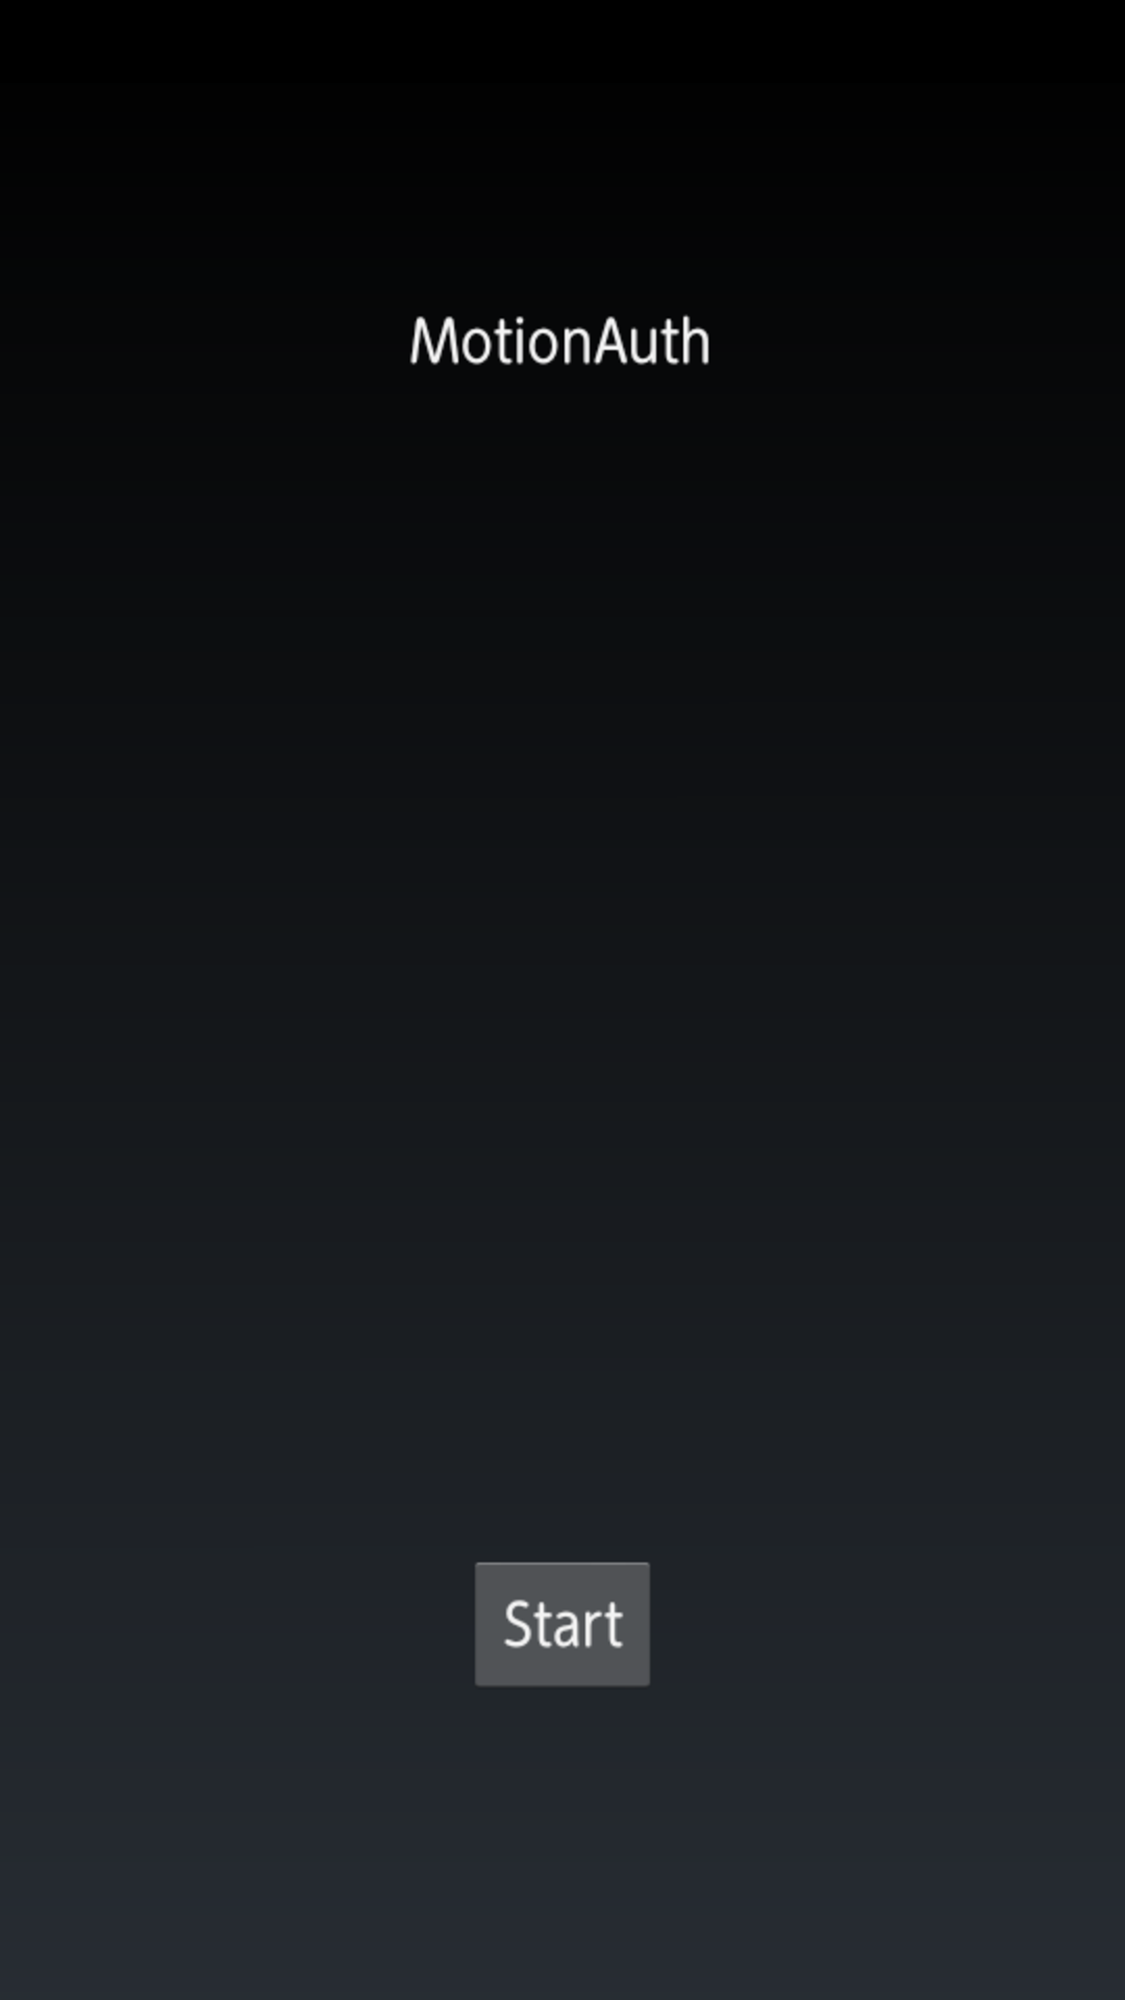
\includegraphics[width=5cm, bb=0 0 540 960]{Start.pdf}
            \end{center}
            \caption{スタート画面}
            \label{start}
        \end{minipage}
        \begin{minipage}{0.5\hsize}
            \begin{center}
                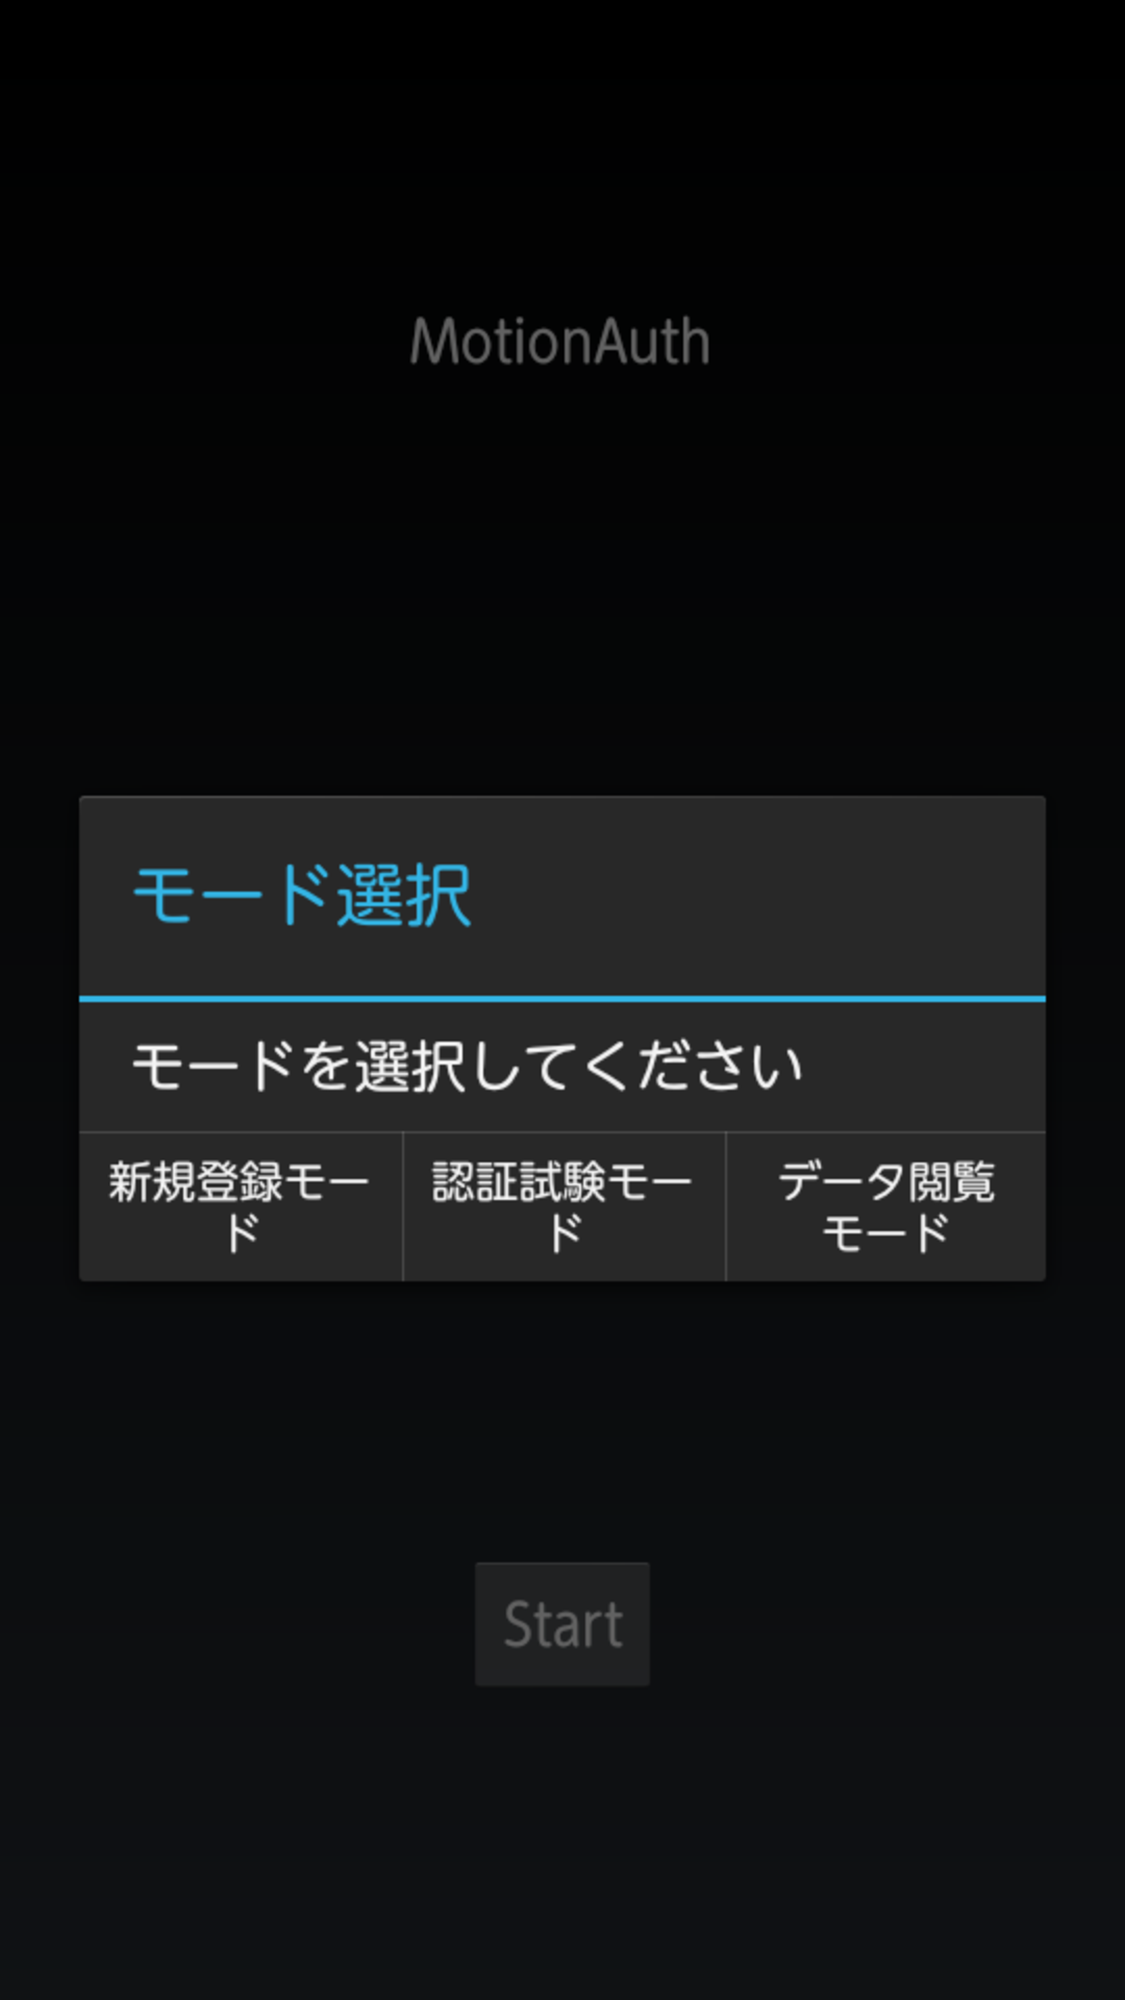
\includegraphics[width=5cm, bb=0 0 540 960]{ModeSelect.pdf}
            \end{center}
            \caption{モード選択ダイアログ}
            \label{selectMode}
        \end{minipage}
    \end{figure}

	    \subsection{新規登録モード}
        新規登録モードでは,まず図\ref{nameInput}の画面にて登録したいユーザの名前を入力させる.
        この画面にてOKボタンを押した際に,テキストフィールドが空であれば,図\ref{nameInputError}のような通知を表示してユーザに名前の再入力を促す.
        テキストフィールドが空でなければ次の図\ref{reg}の画面にてモーションの登録を行わせる.
        OKボタンを押した際の名前の入力値チェックを行うコードをソースコード\ref{checkInputNameSource}に示す.

        % ユーザ名入力画面
        \begin{figure}[htbp]
            \begin{minipage}{0.33\hsize}
                \begin{center}
                    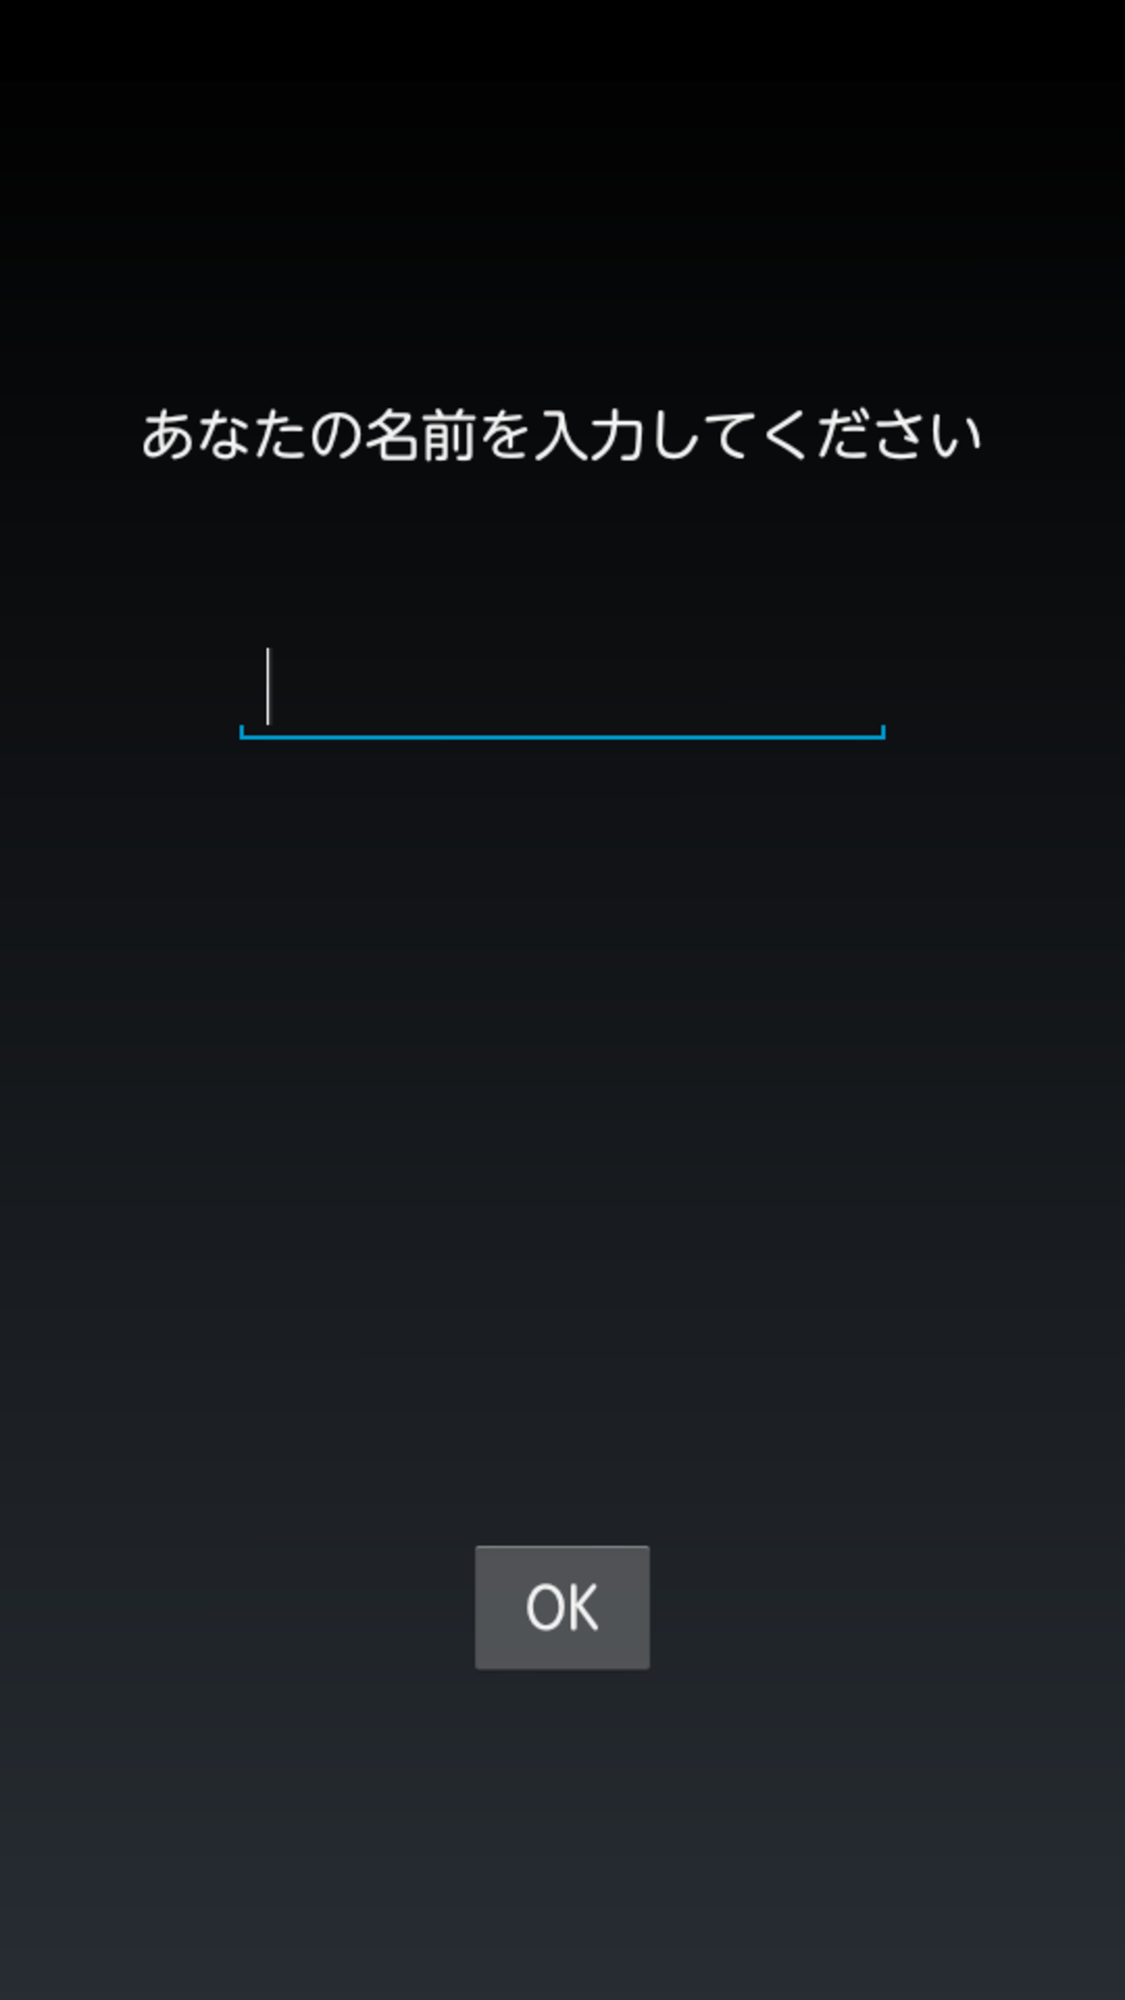
\includegraphics[width=5cm, bb=0 0 540 960]{NameInput.pdf}
                \end{center}
                \caption{ユーザ名入力画面}
                \label{nameInput}
            \end{minipage}
            \begin{minipage}{0.33\hsize}
                \begin{center}
                    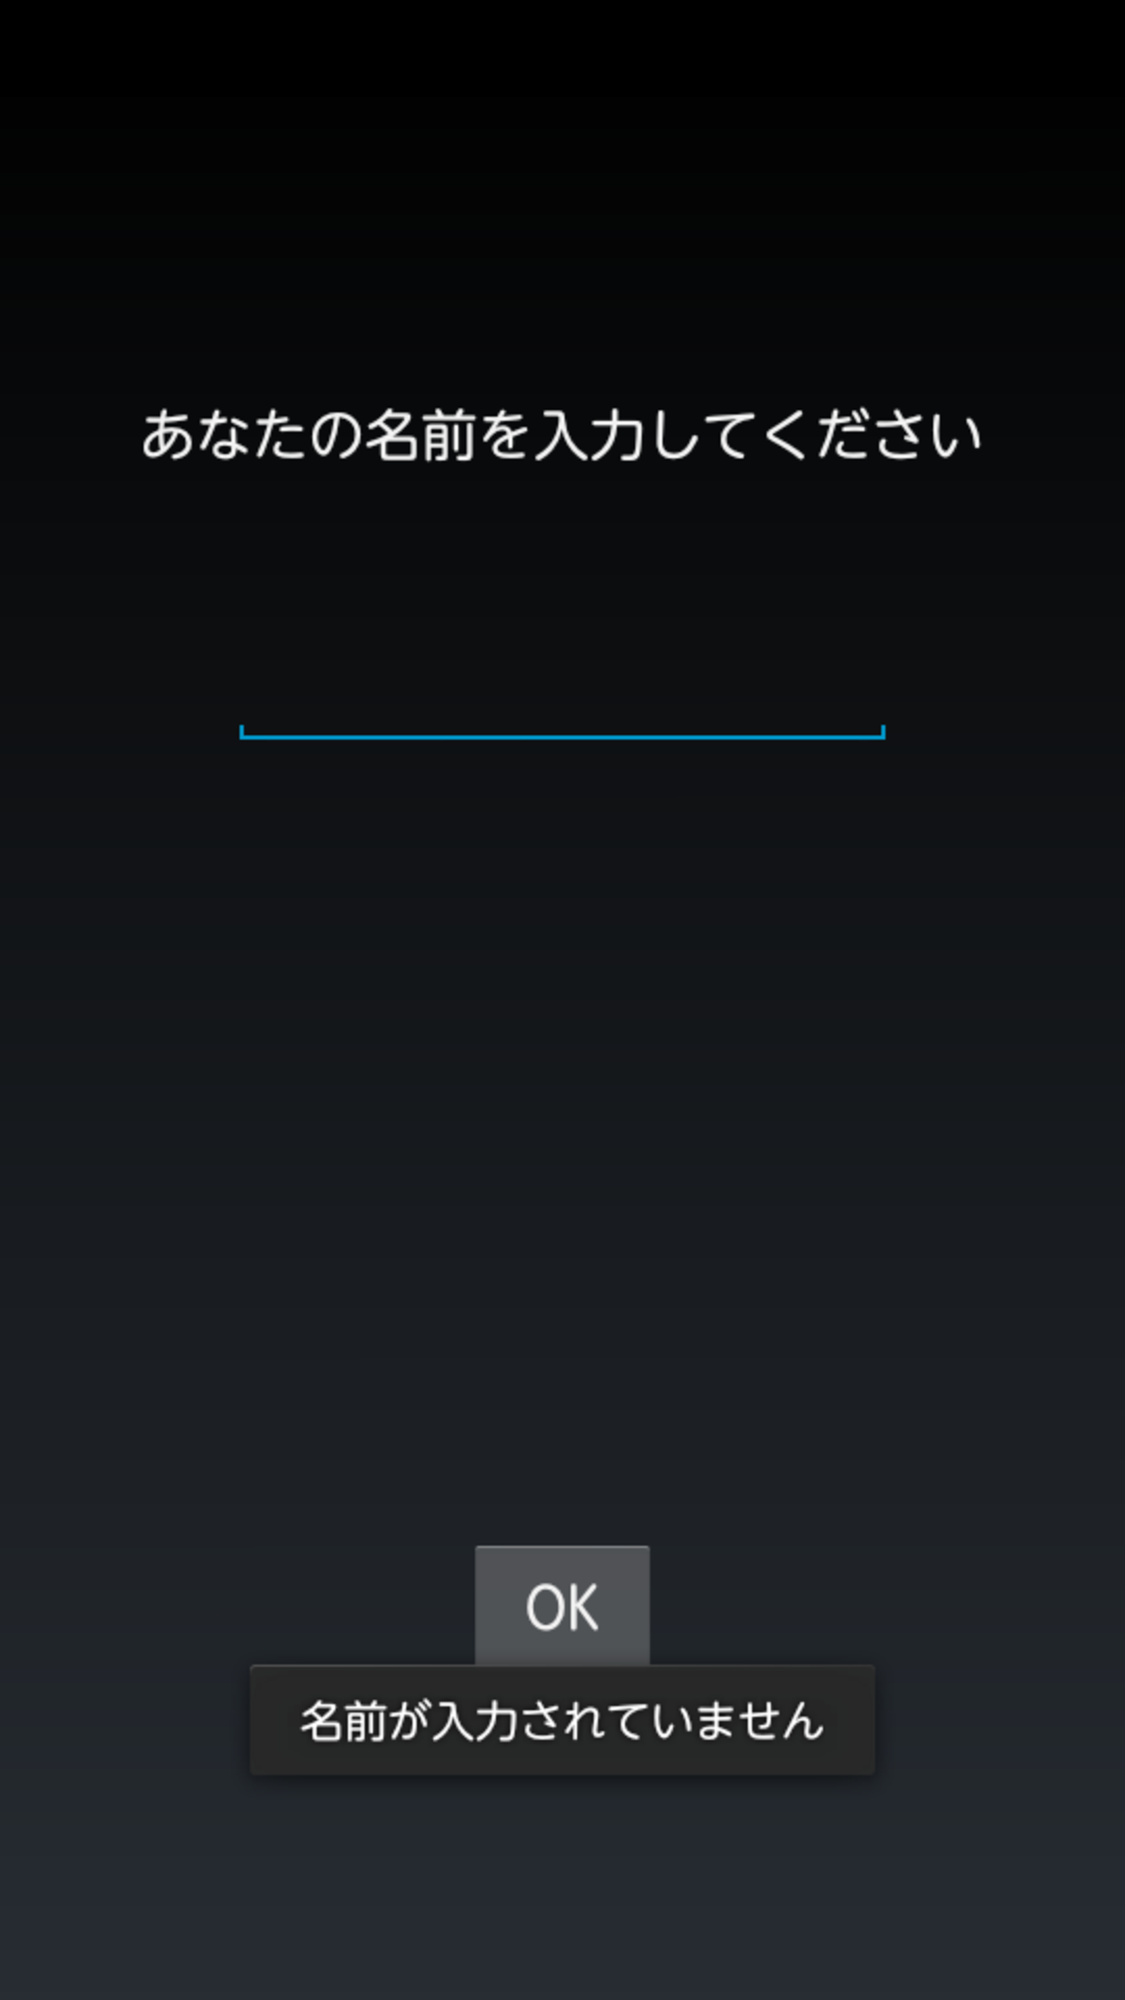
\includegraphics[width=5cm, bb=0 0 540 960]{NameInputError.pdf}
                \end{center}
                \caption{エラー通知}
                \label{nameInputError}
            \end{minipage}
            \begin{minipage}{0.33\hsize}
                \begin{center}
                    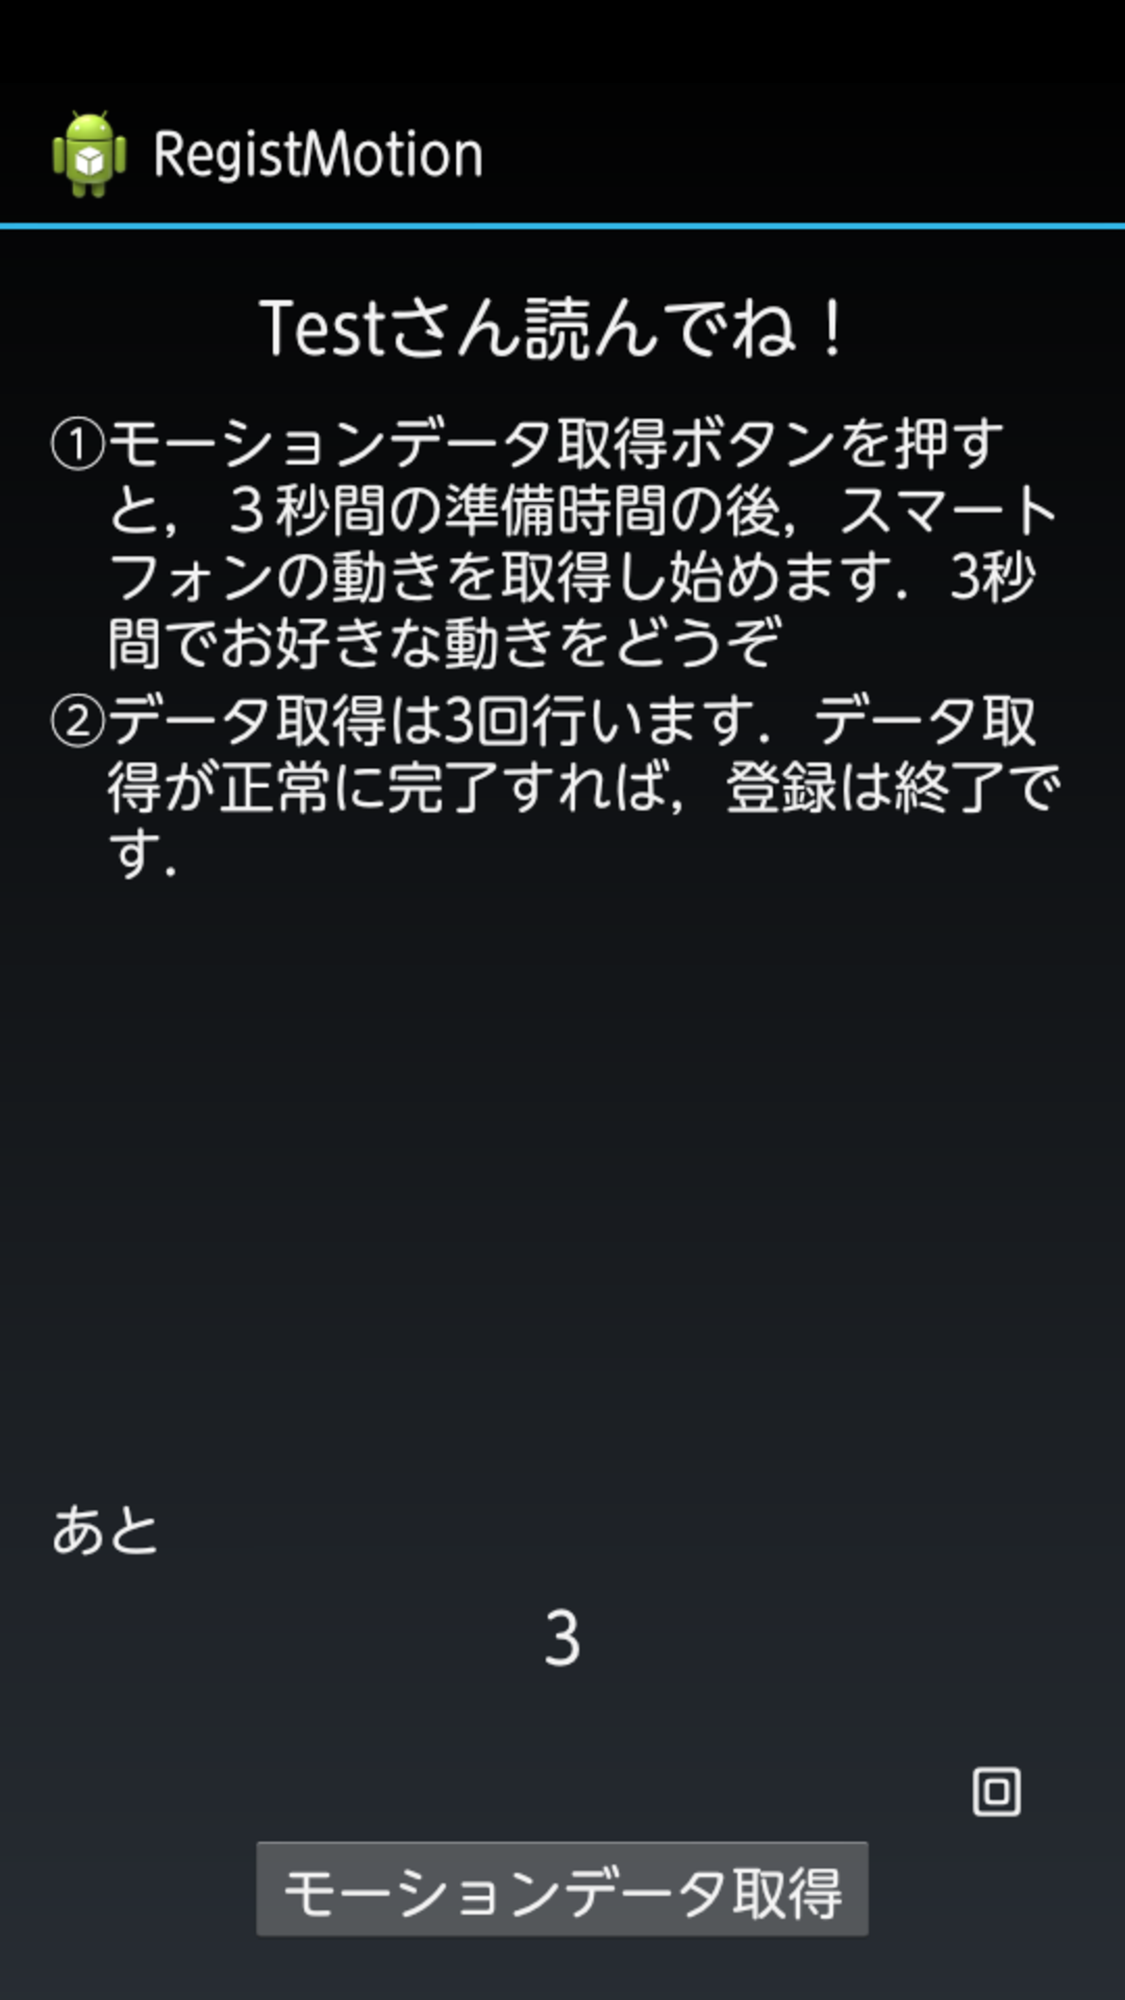
\includegraphics[width=5cm, bb=0 0 540 960]{Reg.pdf}
                \end{center}
                \caption{モーション登録画面}
                \label{reg}
            \end{minipage}
        \end{figure}

        \newpage
        \lstinputlisting[caption=入力値チェック, label=checkInputNameSource]
        {MotionAuth\slash src\slash com\slash example\slash motionauth\slash Registration\slash RegistNameInput.java}
    
        モーションデータ取得ボタンを押すと,三秒間のインターバルを挟んだ後に,モーションデータの取得を三秒間行う.
        この際,画面の下部にそれぞれの経過秒数を表示し,ヴァイブレーションにて一秒毎の時間経過を知らせるようにしている.

        モーションデータの取得は加速度データ,ジャイロデータそれぞれを0.03秒ごとにセンサから取得し,X・Y・Z軸のそれぞれから100個ずつ,計600個を一回分として取得する.

        モーションデータの取得が三回行われると,図\ref{regProgress}のような計算処理待ちダイアログが表示される.
        そして三回分のモーションが同一のモーションであると確認された場合,図\ref{regSuccess}のような登録完了ダイアログが表示され,OKボタンを押すことで取得した三回分のデータの平均値データを保存し,起動画面に移動する.
        また,三回分のモーションが同一のモーションでないと判断された場合,図\ref{regFail}のような登録失敗ダイアログが表示され,OKボタンを押すことでプログラム内部のカウンタが初期化されてデータの取り直しをさせる.

        % モーション登録画面
        \begin{figure}[htbp]
            \begin{minipage}{0.33\hsize}
                \begin{center}
                    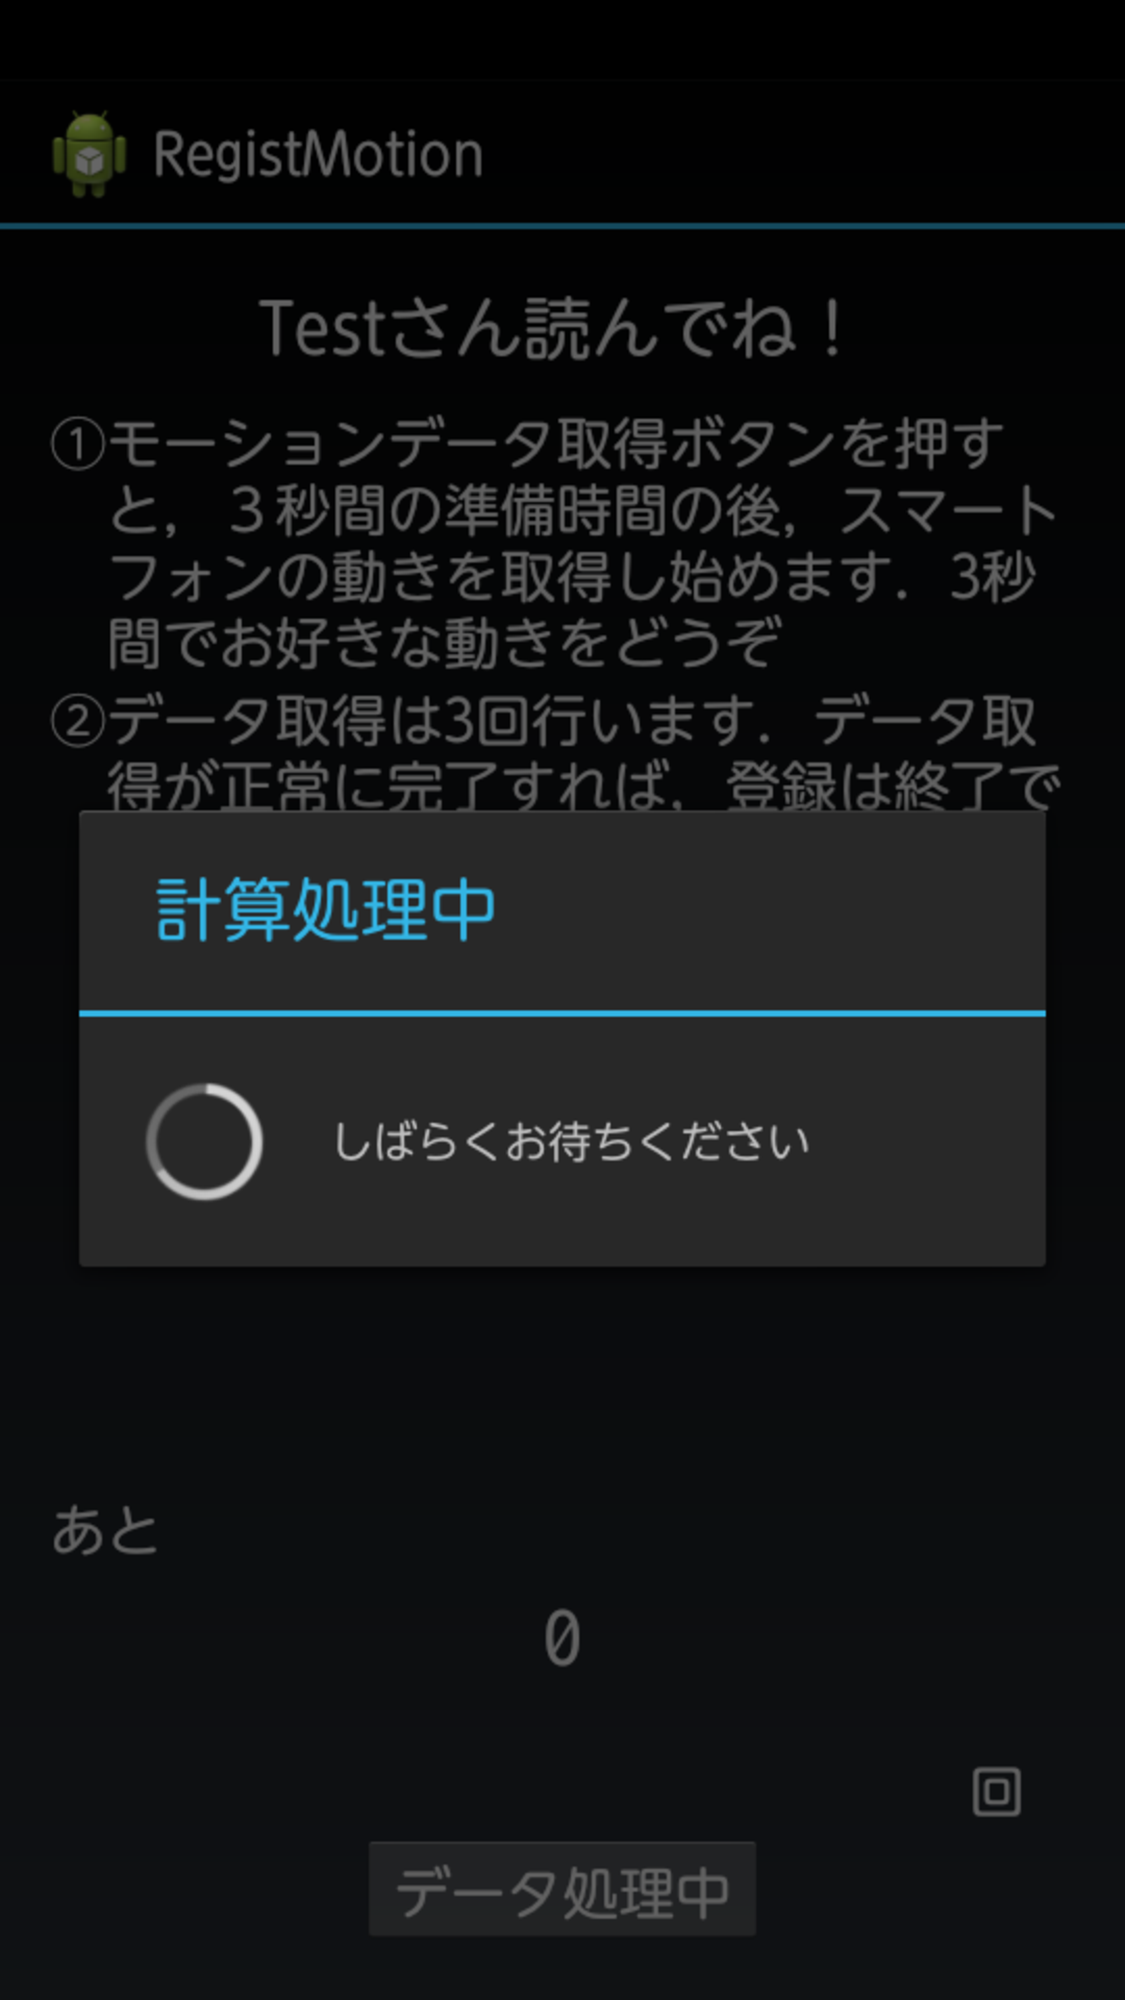
\includegraphics[width=5cm, bb=0 0 540 960]{RegProgress.pdf}
                \end{center}
                \caption{処理待ちダイアログ}
                \label{regProgress}
            \end{minipage}
            \begin{minipage}{0.33\hsize}
                \begin{center}
                    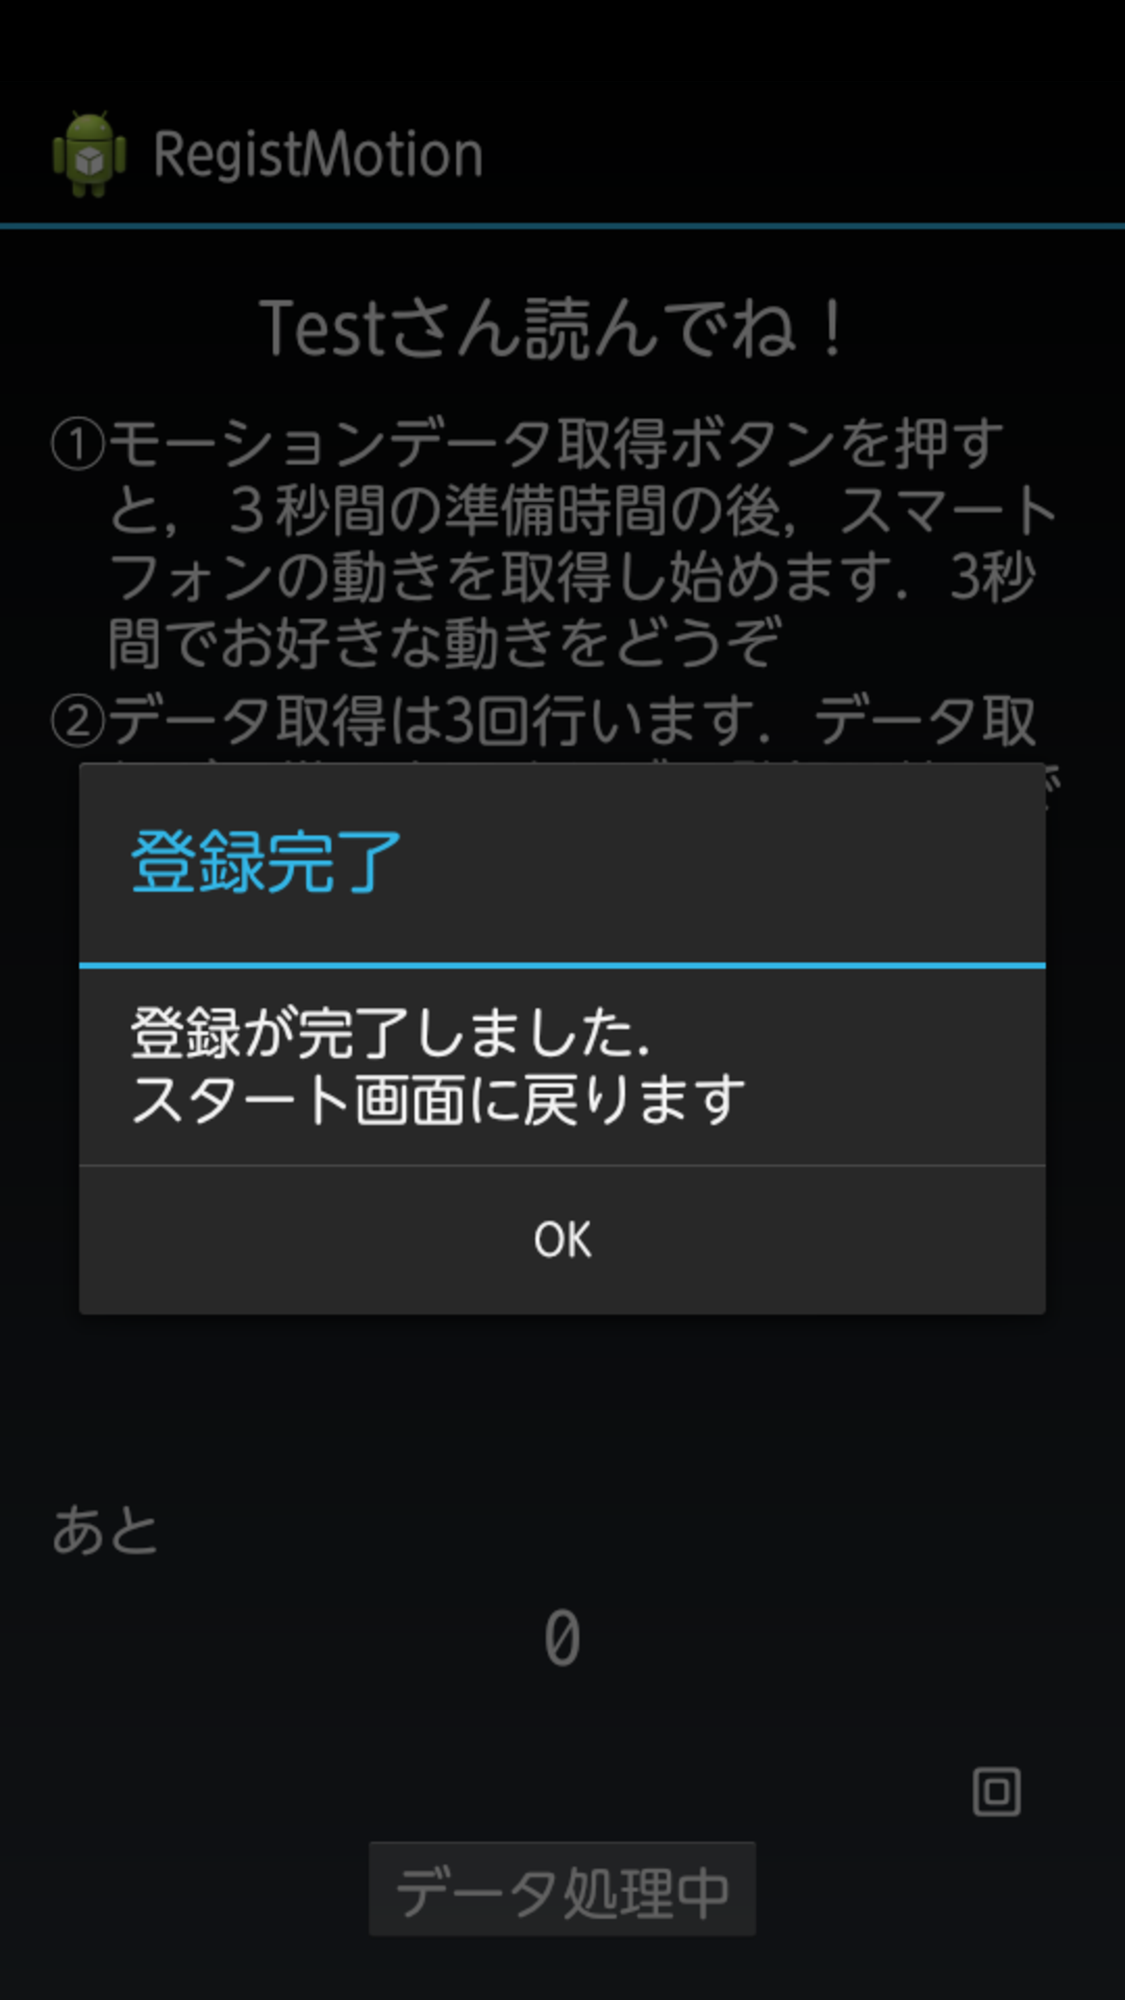
\includegraphics[width=5cm, bb=0 0 540 960]{RegSuccess.pdf}
                \end{center}
                \caption{登録完了ダイアログ}
                \label{regSuccess}
            \end{minipage}
            \begin{minipage}{0.33\hsize}
                \begin{center}
                    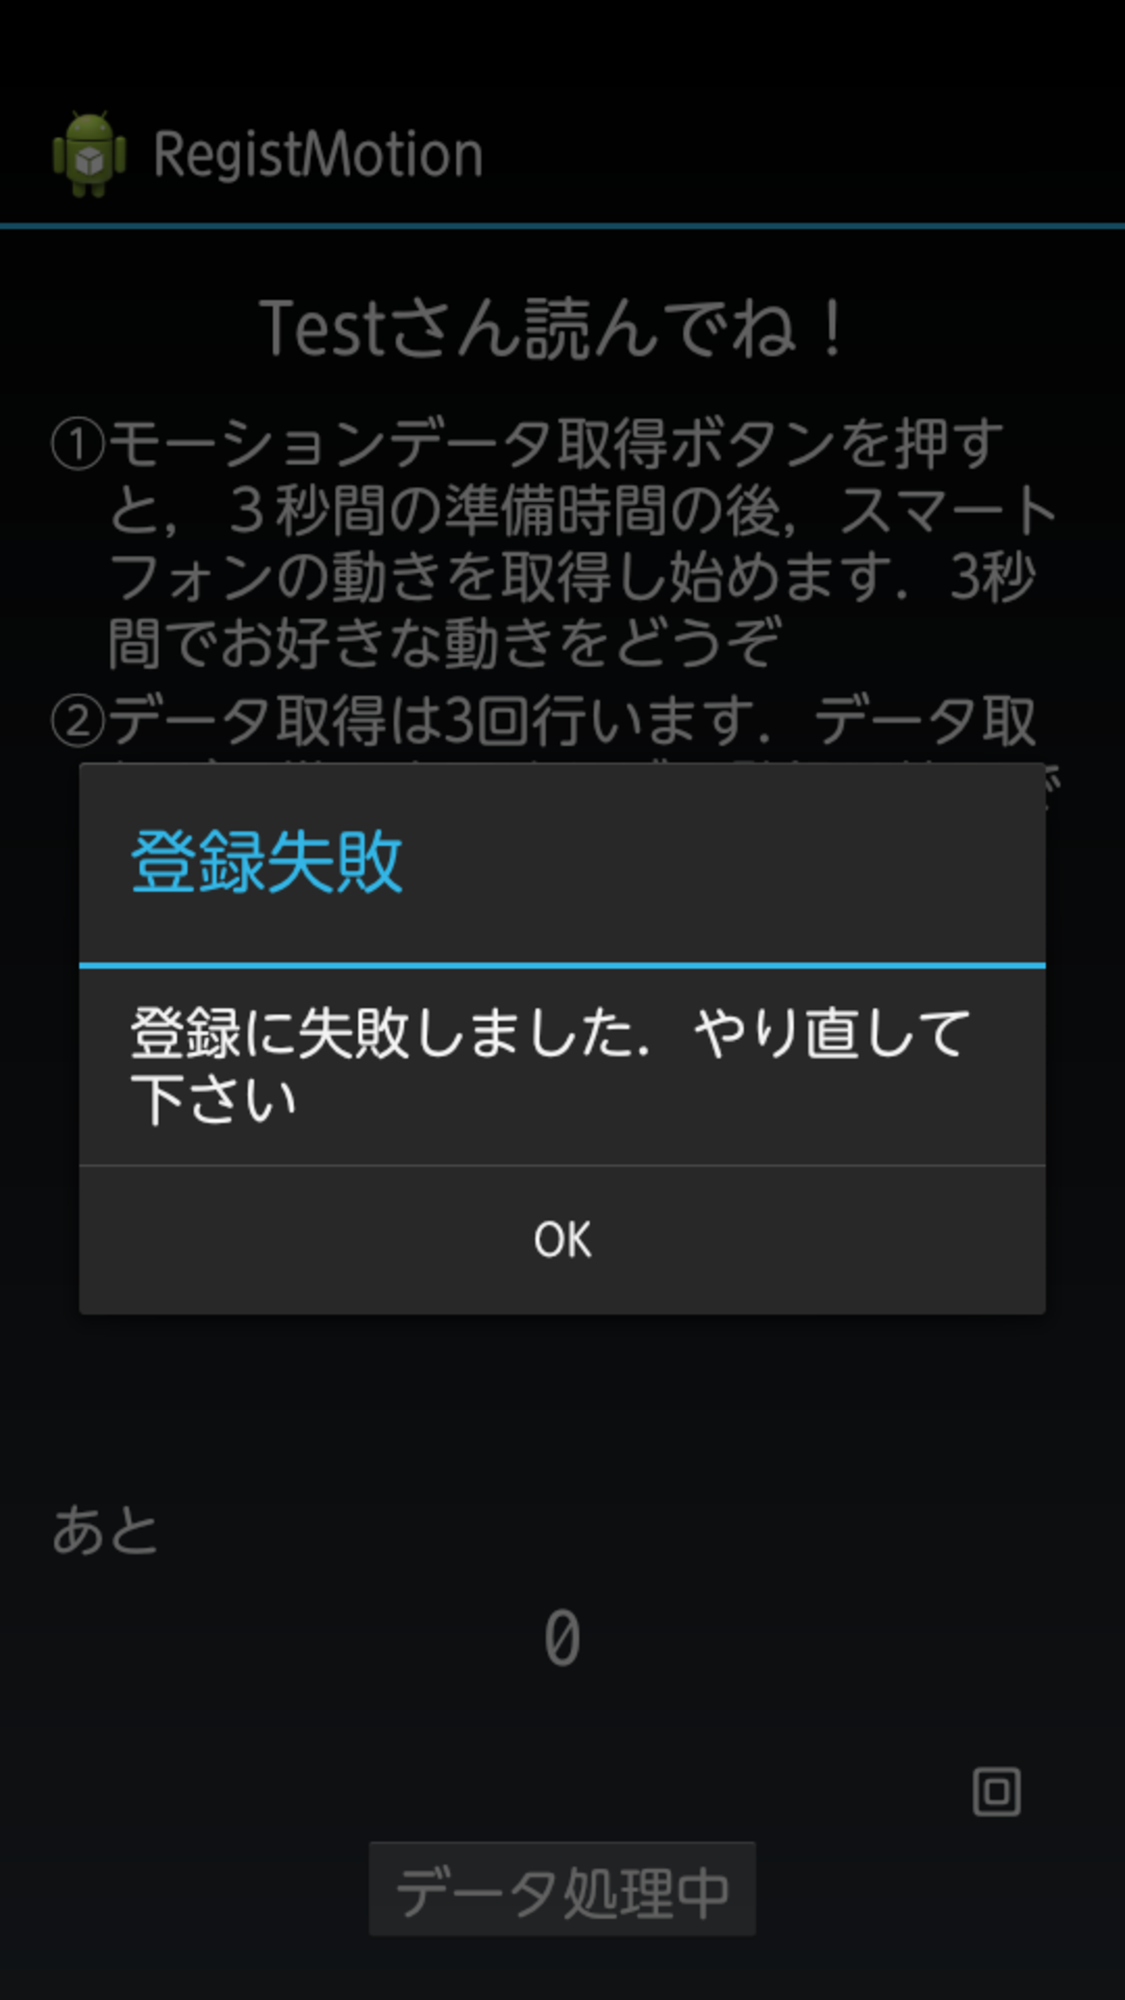
\includegraphics[width=5cm, bb=0 0 540 960]{RegFail.pdf}
                \end{center}
                \caption{登録失敗ダイアログ}
                \label{regFail}
            \end{minipage}
        \end{figure}

        \newpage
	    \subsection{認証試験モード}
        認証試験モードでは,図\ref{authNameInput}の画面にて,新規登録モードであらかじめ登録されたユーザ名を入力させる.
        指定されたユーザ名にて既にモーションの登録がなされていることが確認できた場合にのみ,図\ref{auth}の画面にて個人認証を行わせる.
        モーションの登録がなされていなかった場合,図\ref{authNameInputError}のようなダイアログを表示する.

        \begin{figure}[htbp]
            \begin{minipage}{0.33\hsize}
                \begin{center}
                    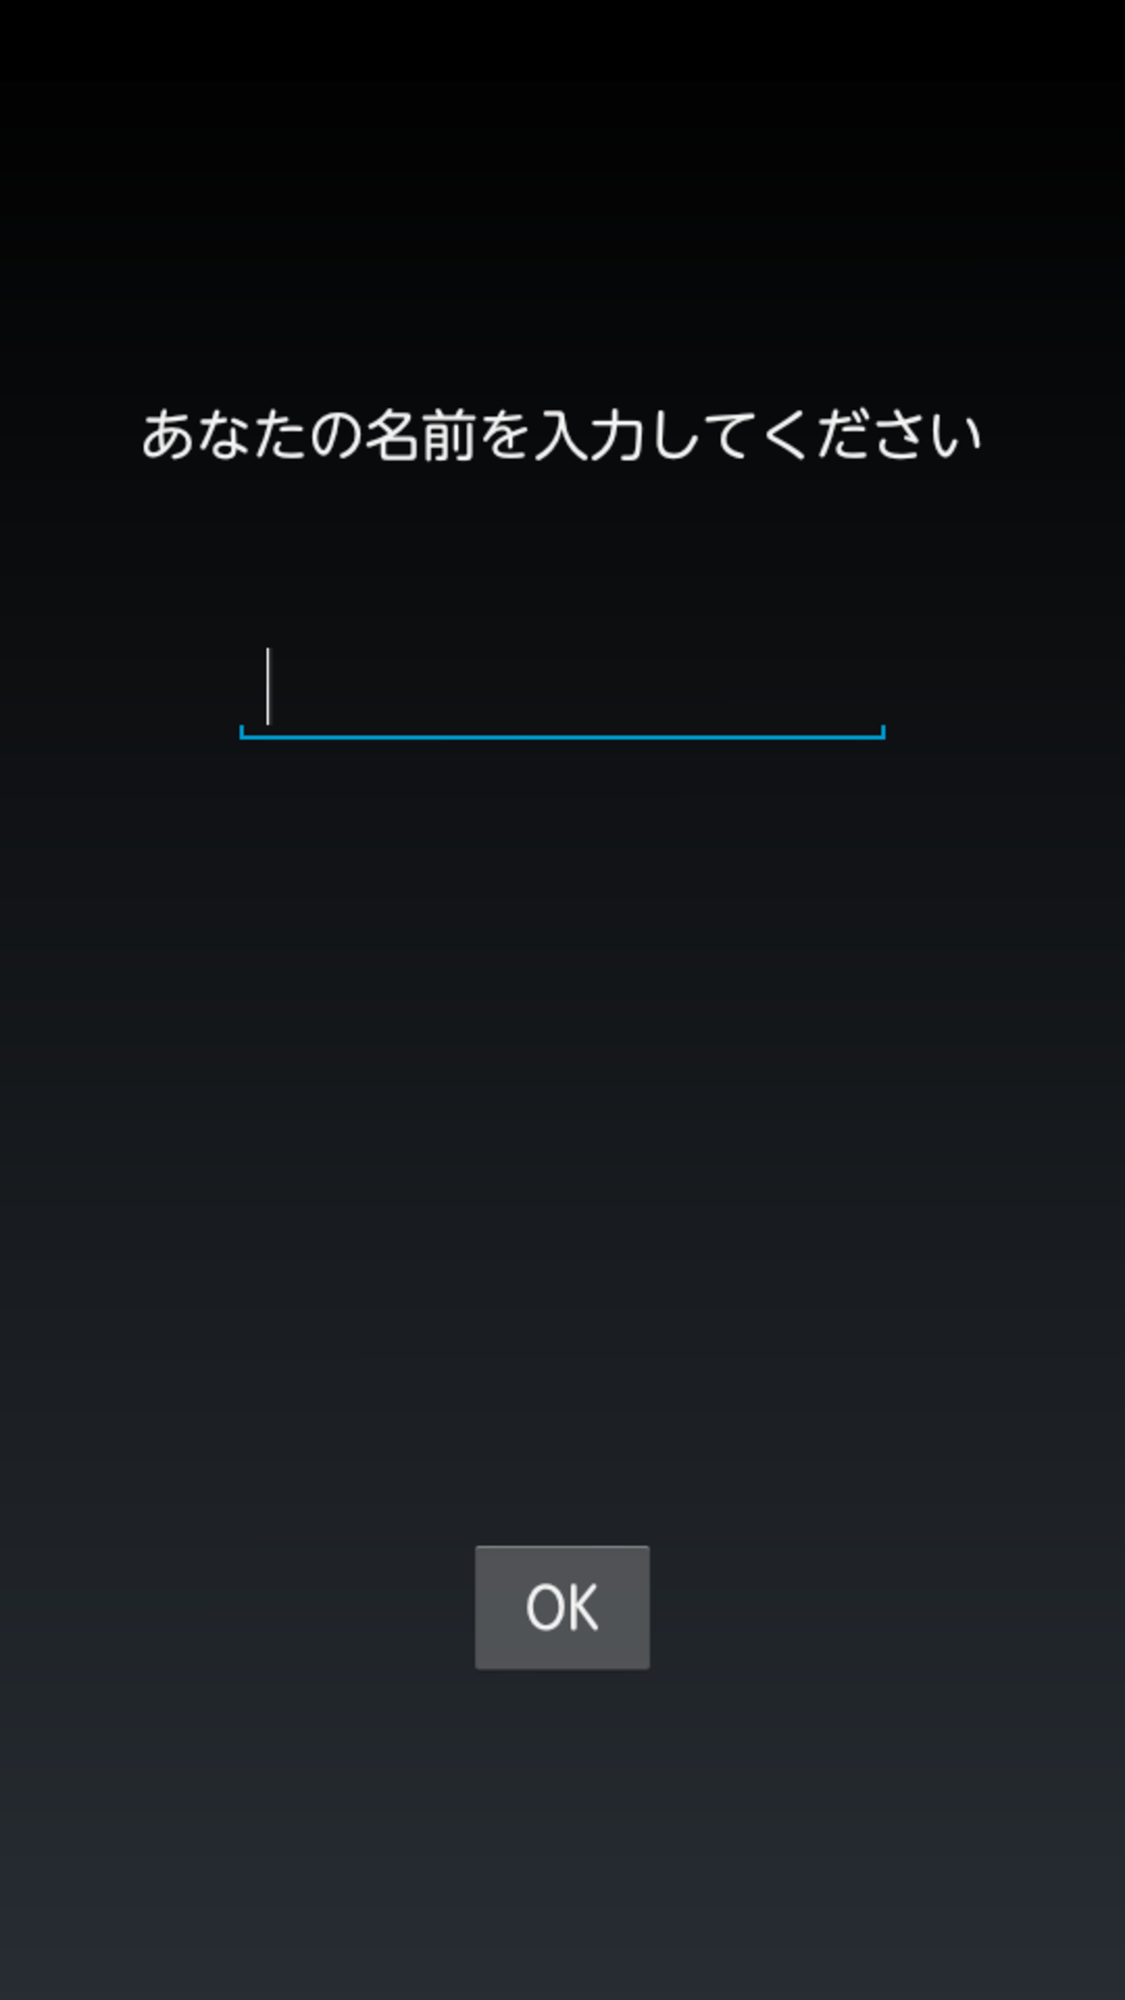
\includegraphics[width=5cm, bb=0 0 540 960]{NameInput.pdf}
                \end{center}
                \caption{ユーザ名入力画面}
                \label{authNameInput}
            \end{minipage}
            \begin{minipage}{0.33\hsize}
                \begin{center}
                    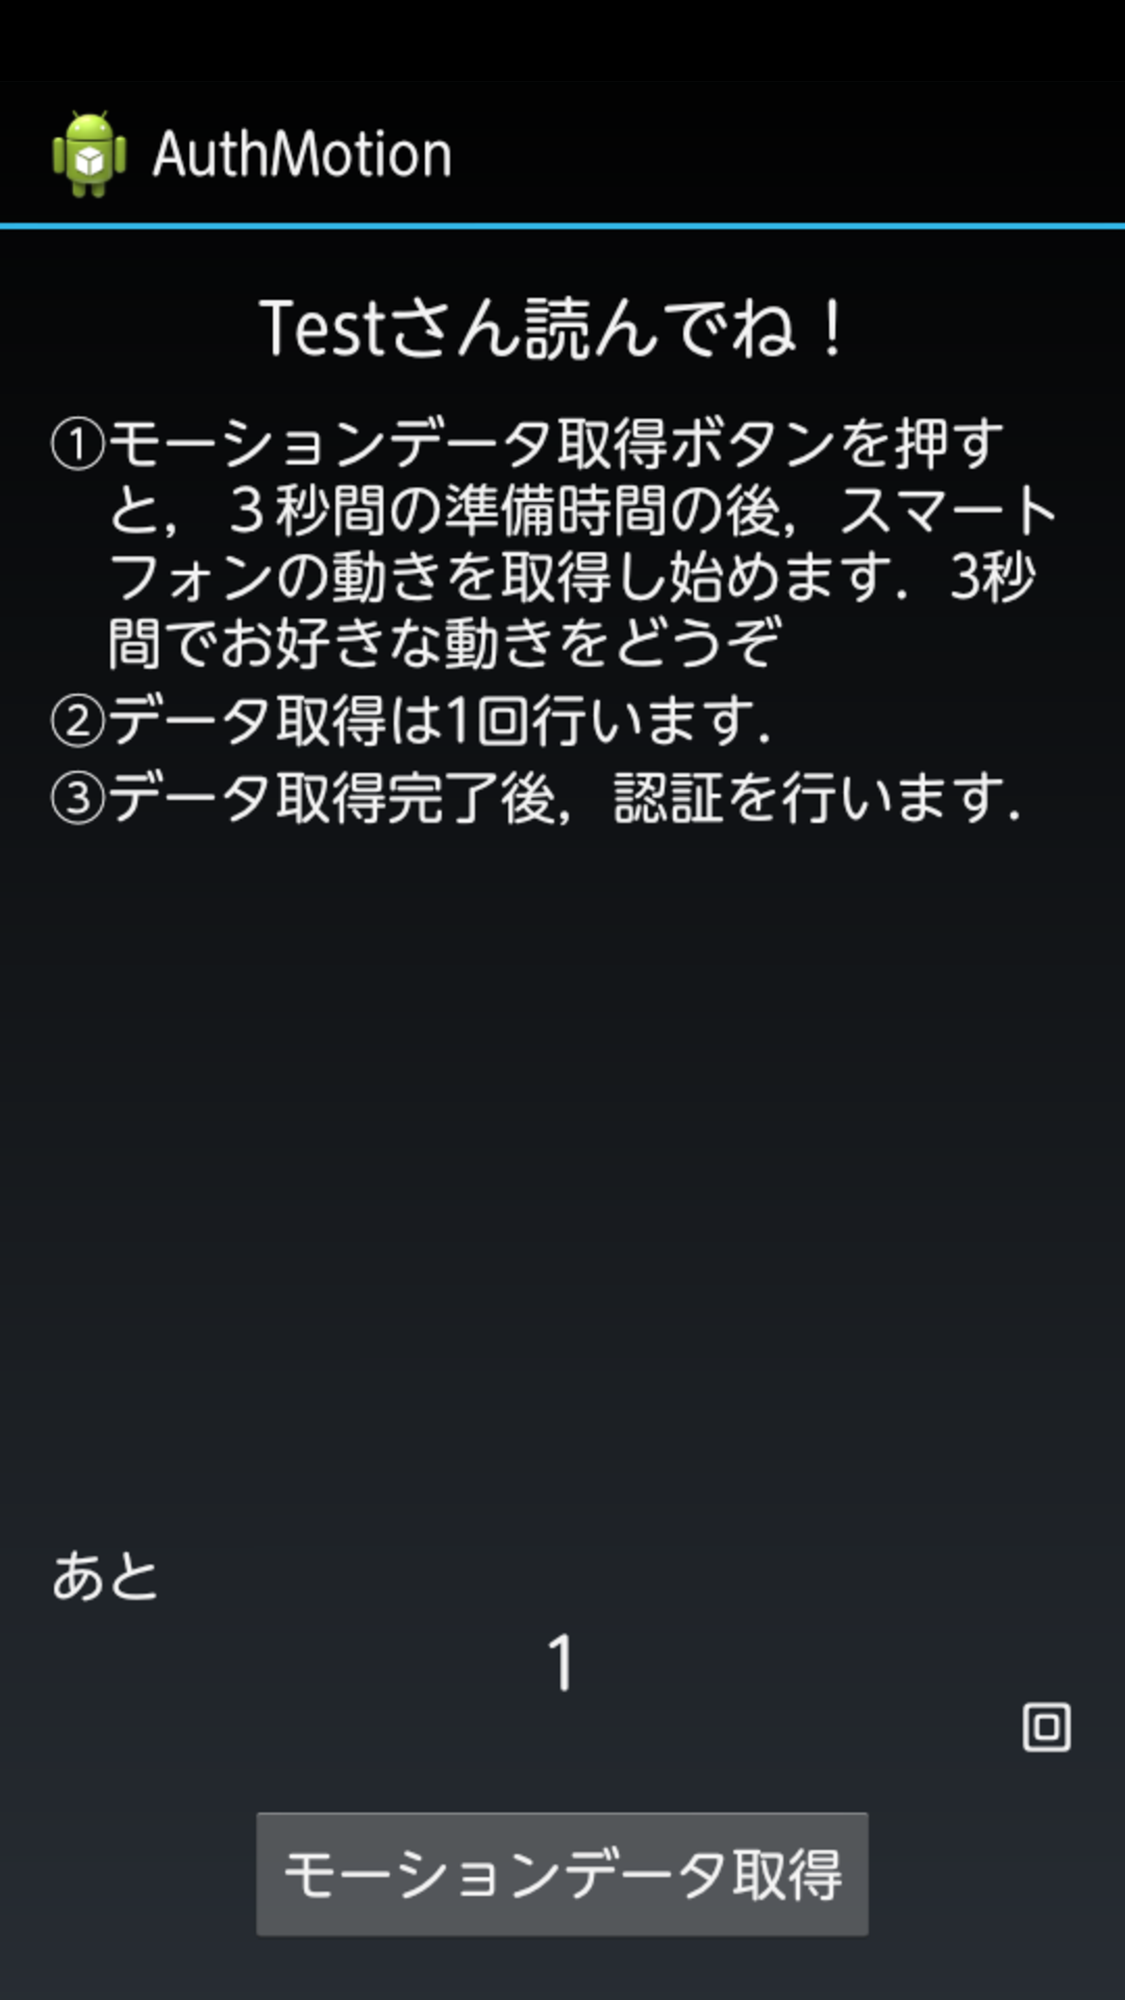
\includegraphics[width=5cm, bb=0 0 540 960]{Auth.pdf}
                \end{center}
                \caption{認証試験画面}
                \label{auth}
            \end{minipage}
            \begin{minipage}{0.33\hsize}
                \begin{center}
                    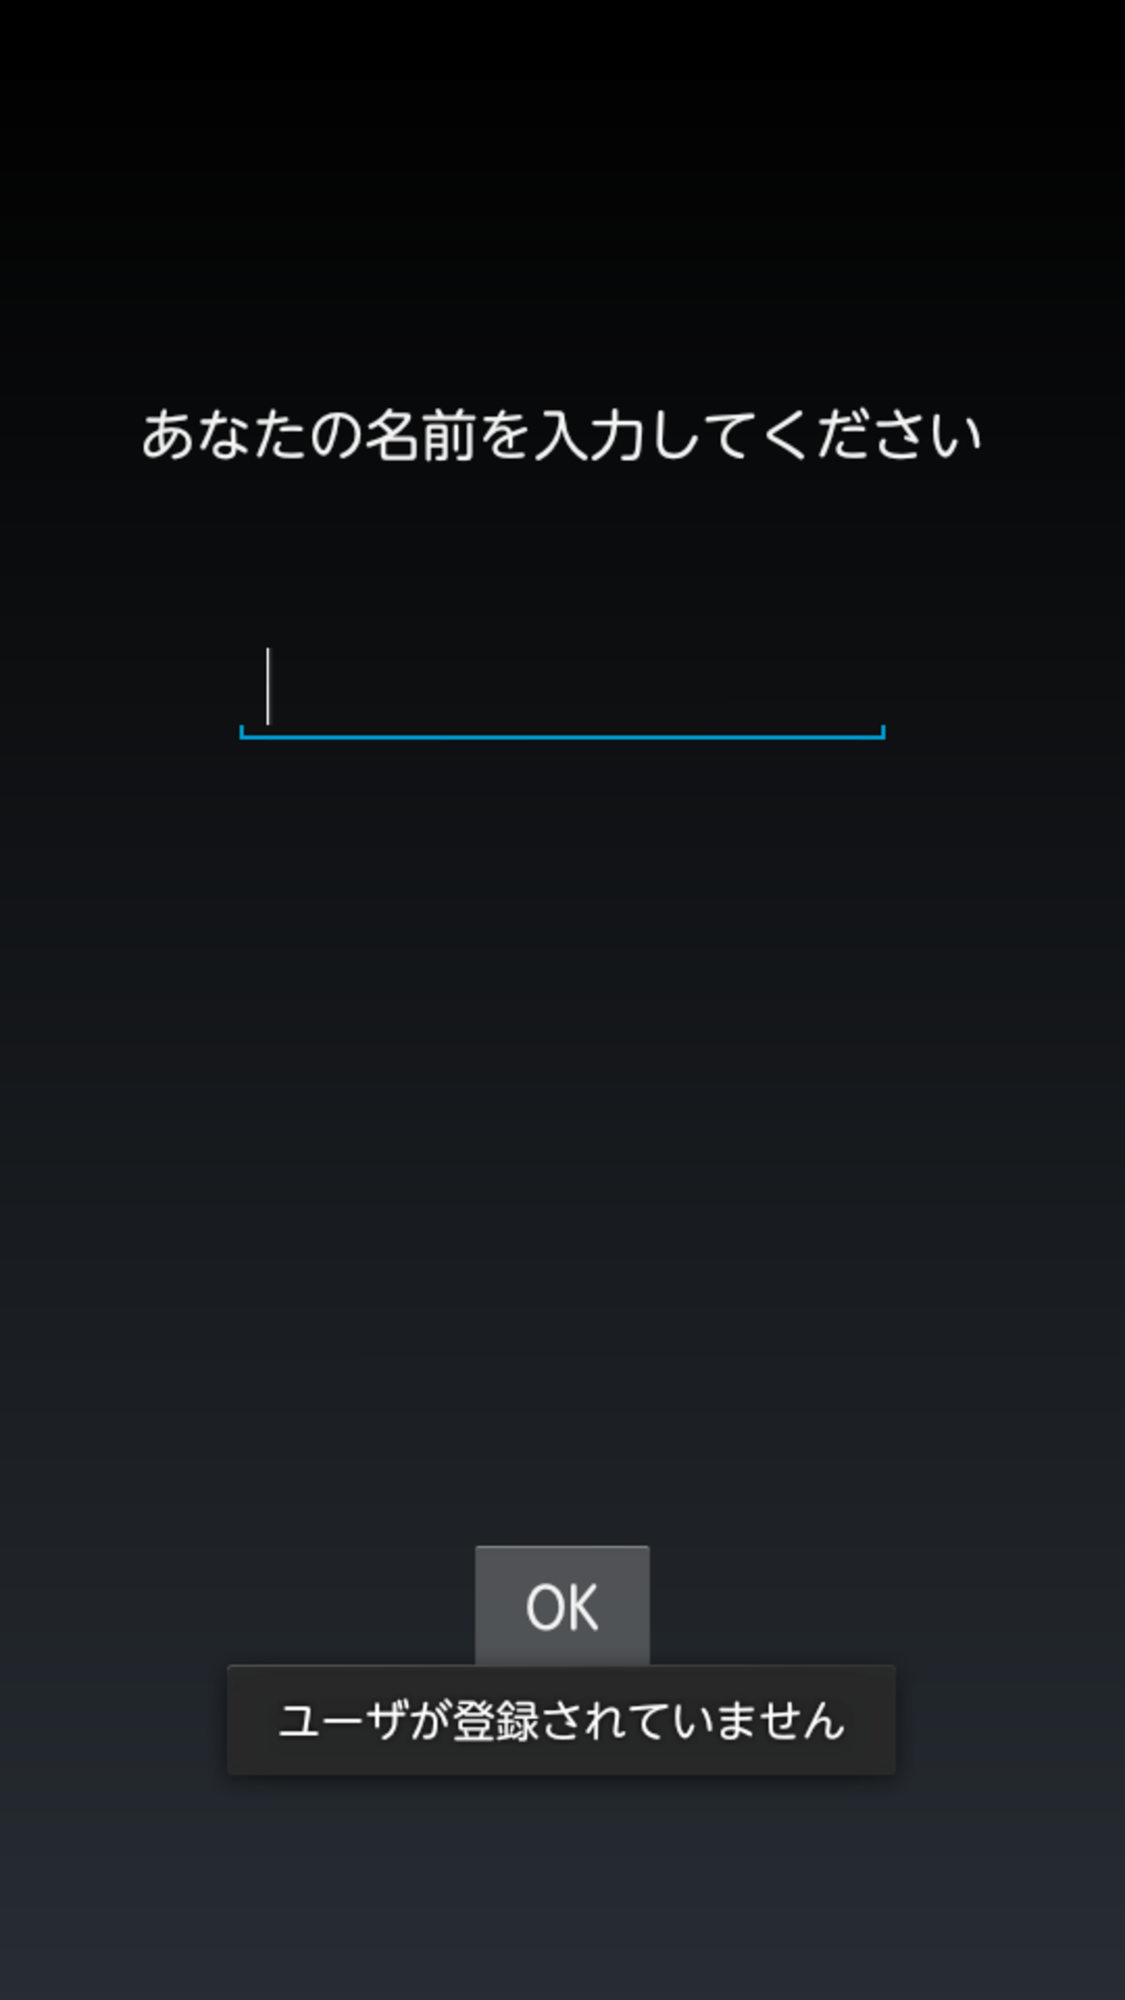
\includegraphics[width=5cm, bb=0 0 540 960]{AuthNameInputError.pdf}
                \end{center}
                \caption{エラー通知}
                \label{authNameInputError}
            \end{minipage}
        \end{figure}

        認証試験モードでは新規登録モードとは異なり,一回分のみのモーションデータ取得を行わせる.
        モーションデータの取得後,新規登録モードにて登録されたモーションデータを読み出し,これと新たに入力させたモーションとの相関を取ることで個人認証を行う.
        認証に成功すれば図\ref{authSuccess}のような認証成功ダイアログを表示し,OKボタンを押すことで起動画面へ移動する.
        認証に失敗すれば図\ref{authFail}のような認証失敗ダイアログを表示し,OKボタンを押すことで内部のカウンタを初期化して再度認証を行えるようにする.

        \begin{figure}[htbp]
            \begin{minipage}{0.5\hsize}
                \begin{center}
                    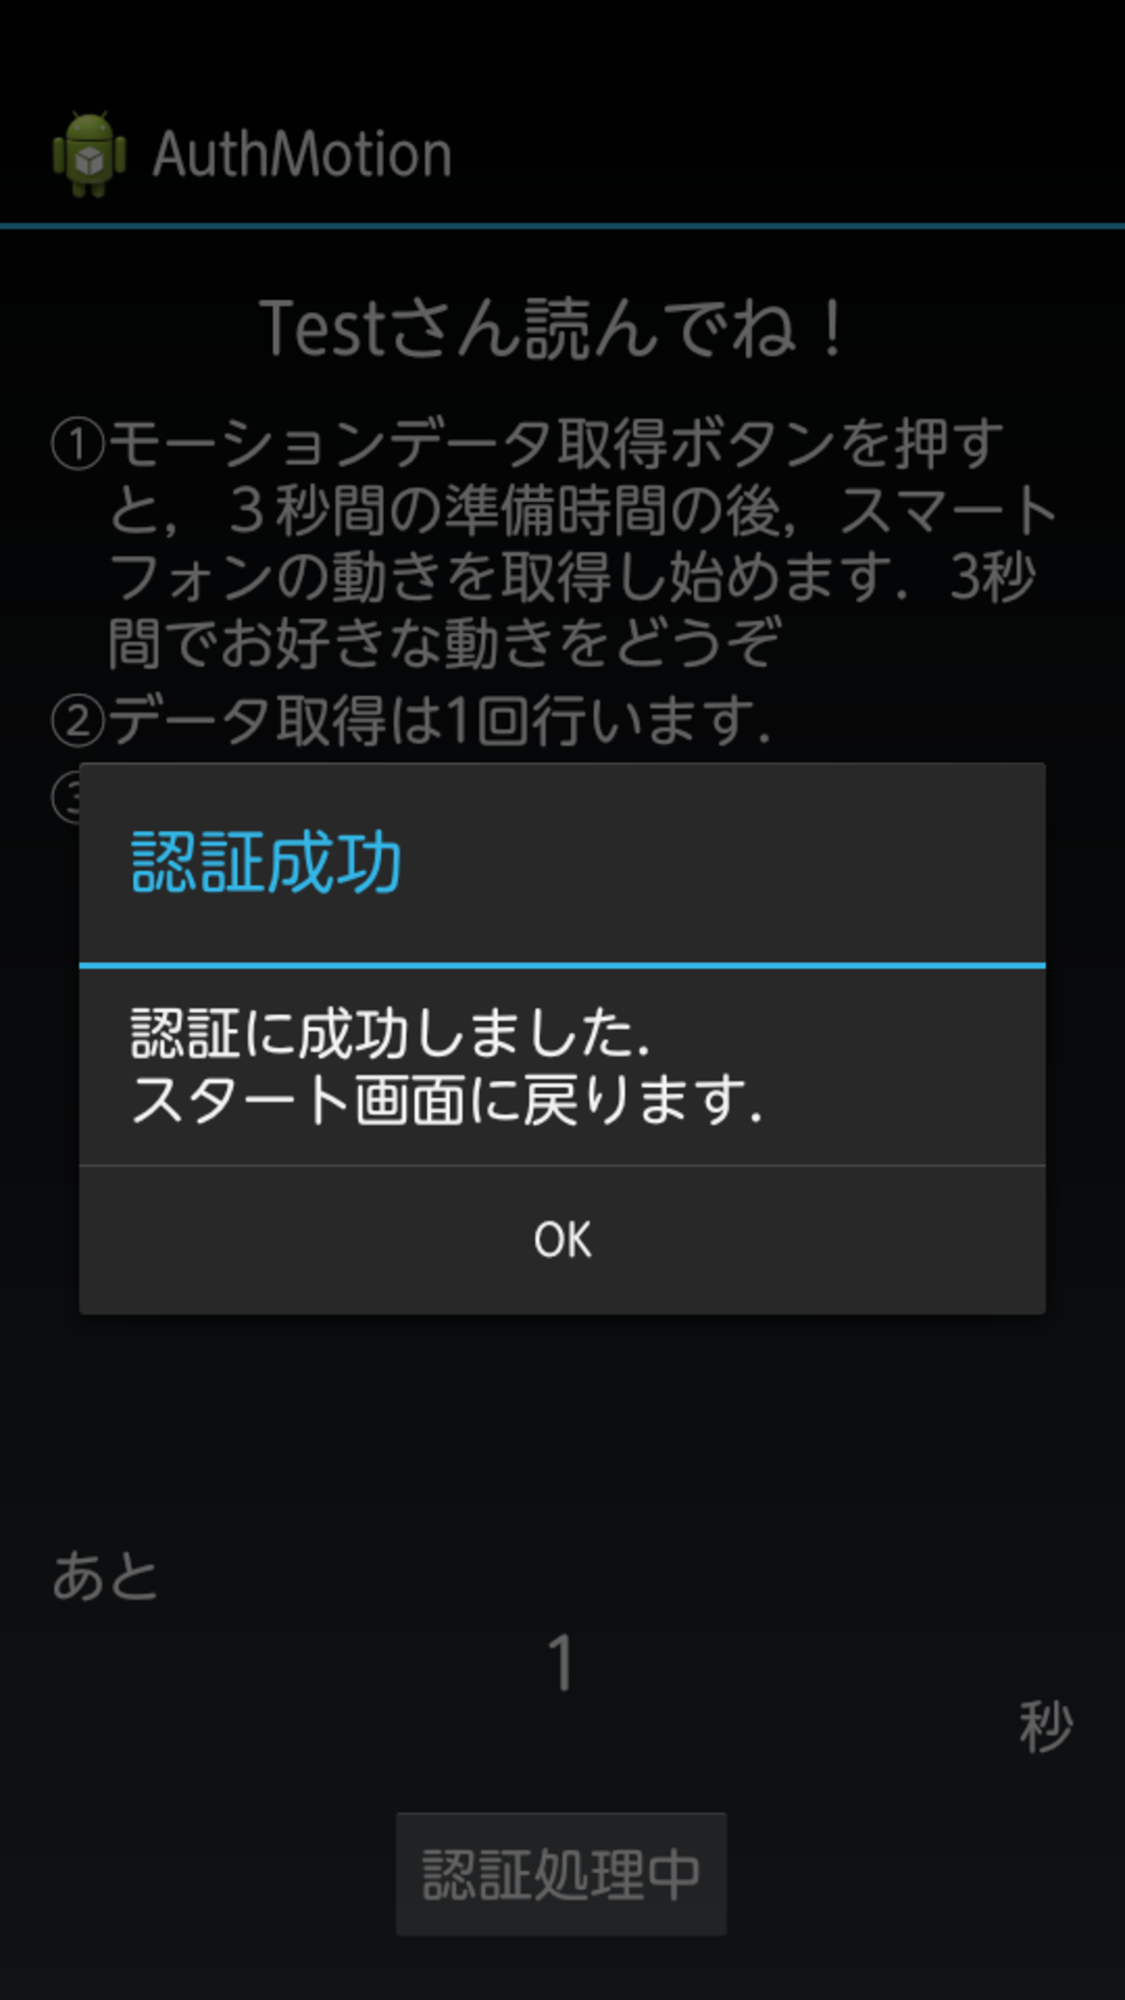
\includegraphics[width=5cm, bb=0 0 540 960]{AuthSuccess.pdf}
                \end{center}
                \caption{認証成功ダイアログ}
                \label{authSuccess}
            \end{minipage}
            \begin{minipage}{0.5\hsize}
                \begin{center}
                    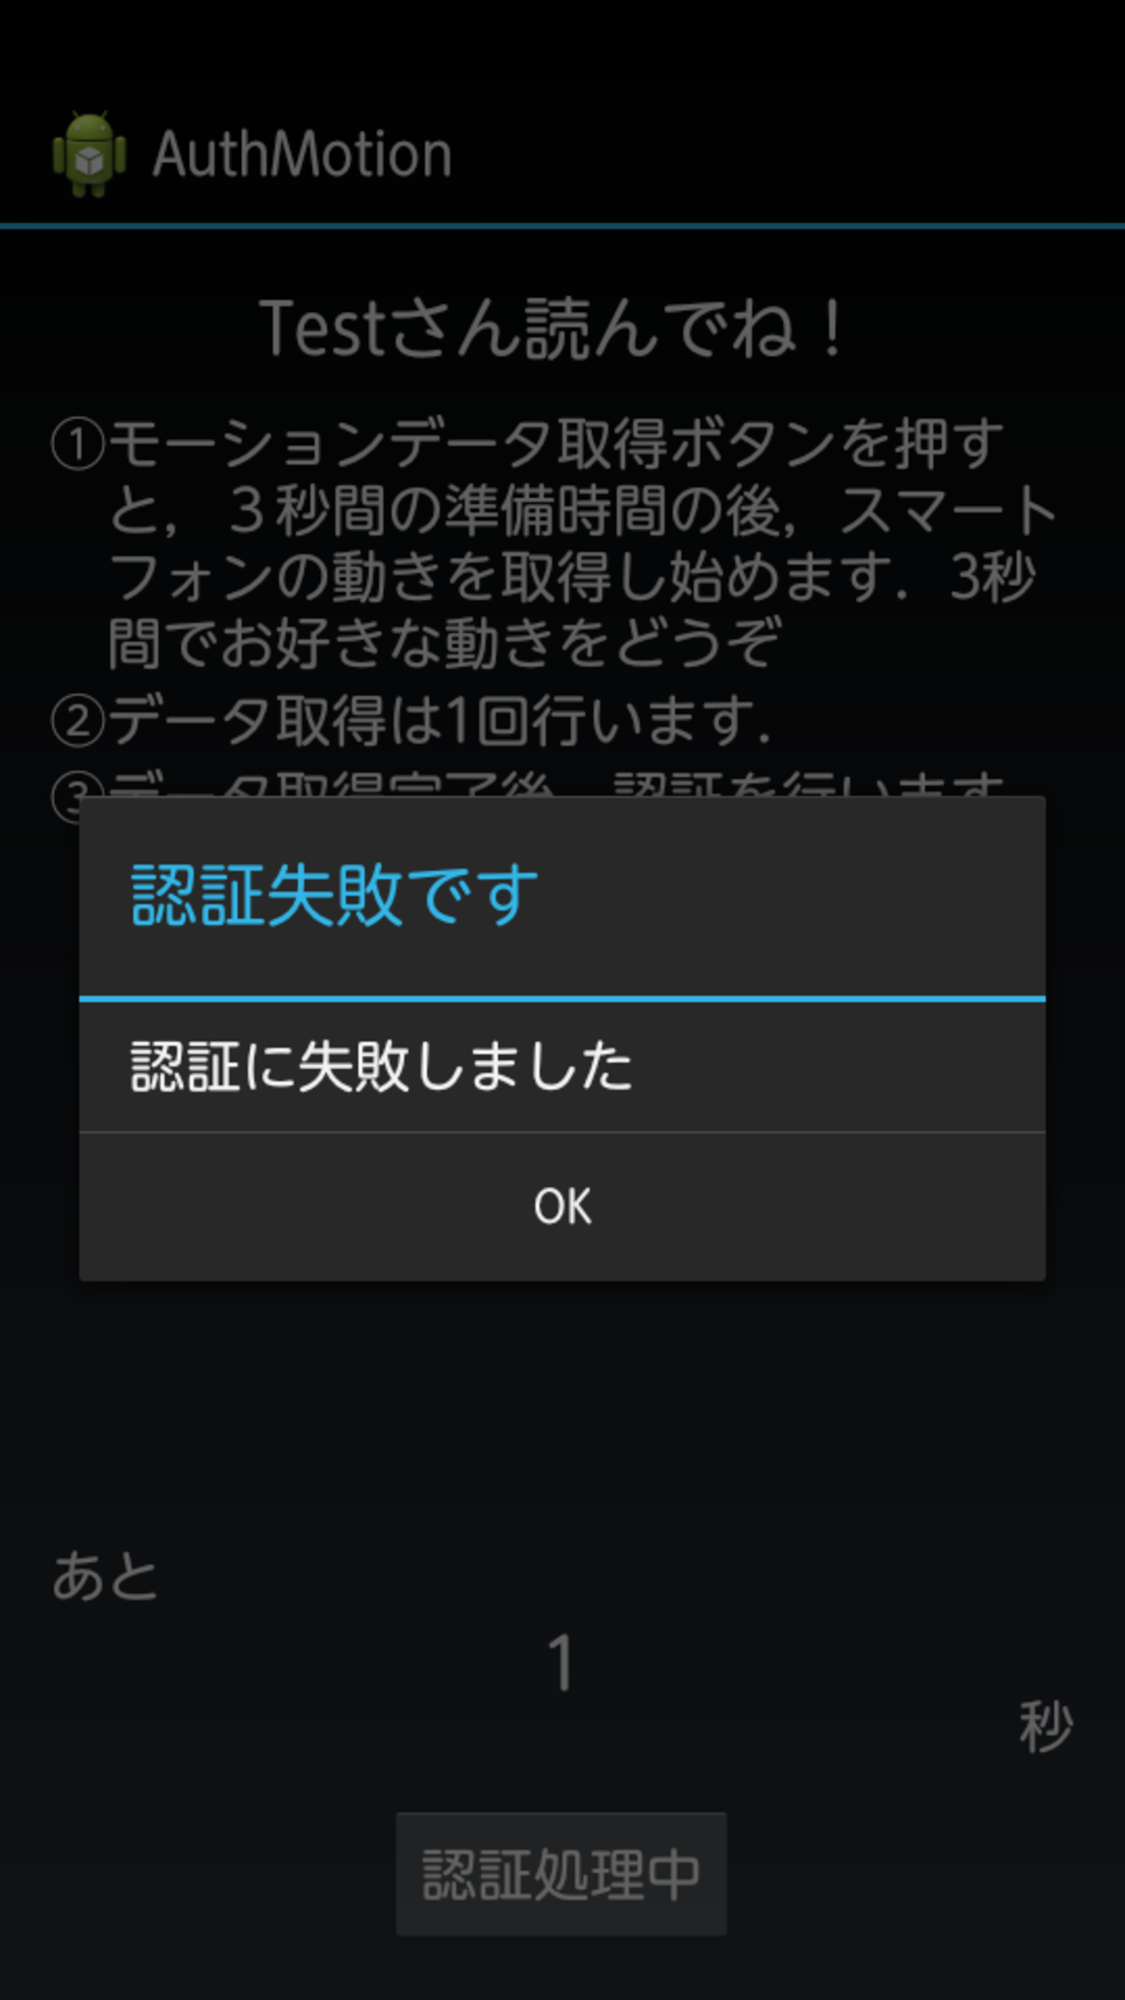
\includegraphics[width=5cm, bb=0 0 540 960]{AuthFail.pdf}
                \end{center}
                \caption{認証失敗ダイアログ}
                \label{authFail}
            \end{minipage}
        \end{figure}

	    \subsection{データ閲覧モード}
	    データ閲覧モードでは,新規登録モードにて登録されたユーザ名を一覧で見ることが出来る.
        また,その中からユーザ名を選択するとそのユーザが登録したモーションデータを見ることが出来る.
        このモードを選択すると,まず図\ref{userList}のようなユーザ名の一覧が表示される.
        ここでデータを閲覧したいユーザ名を選択することで,図\ref{dataList}のようなモーションデータ一覧が表示される.

        \begin{figure}[htbp]
            \begin{minipage}{0.5\hsize}
                \begin{center}
                    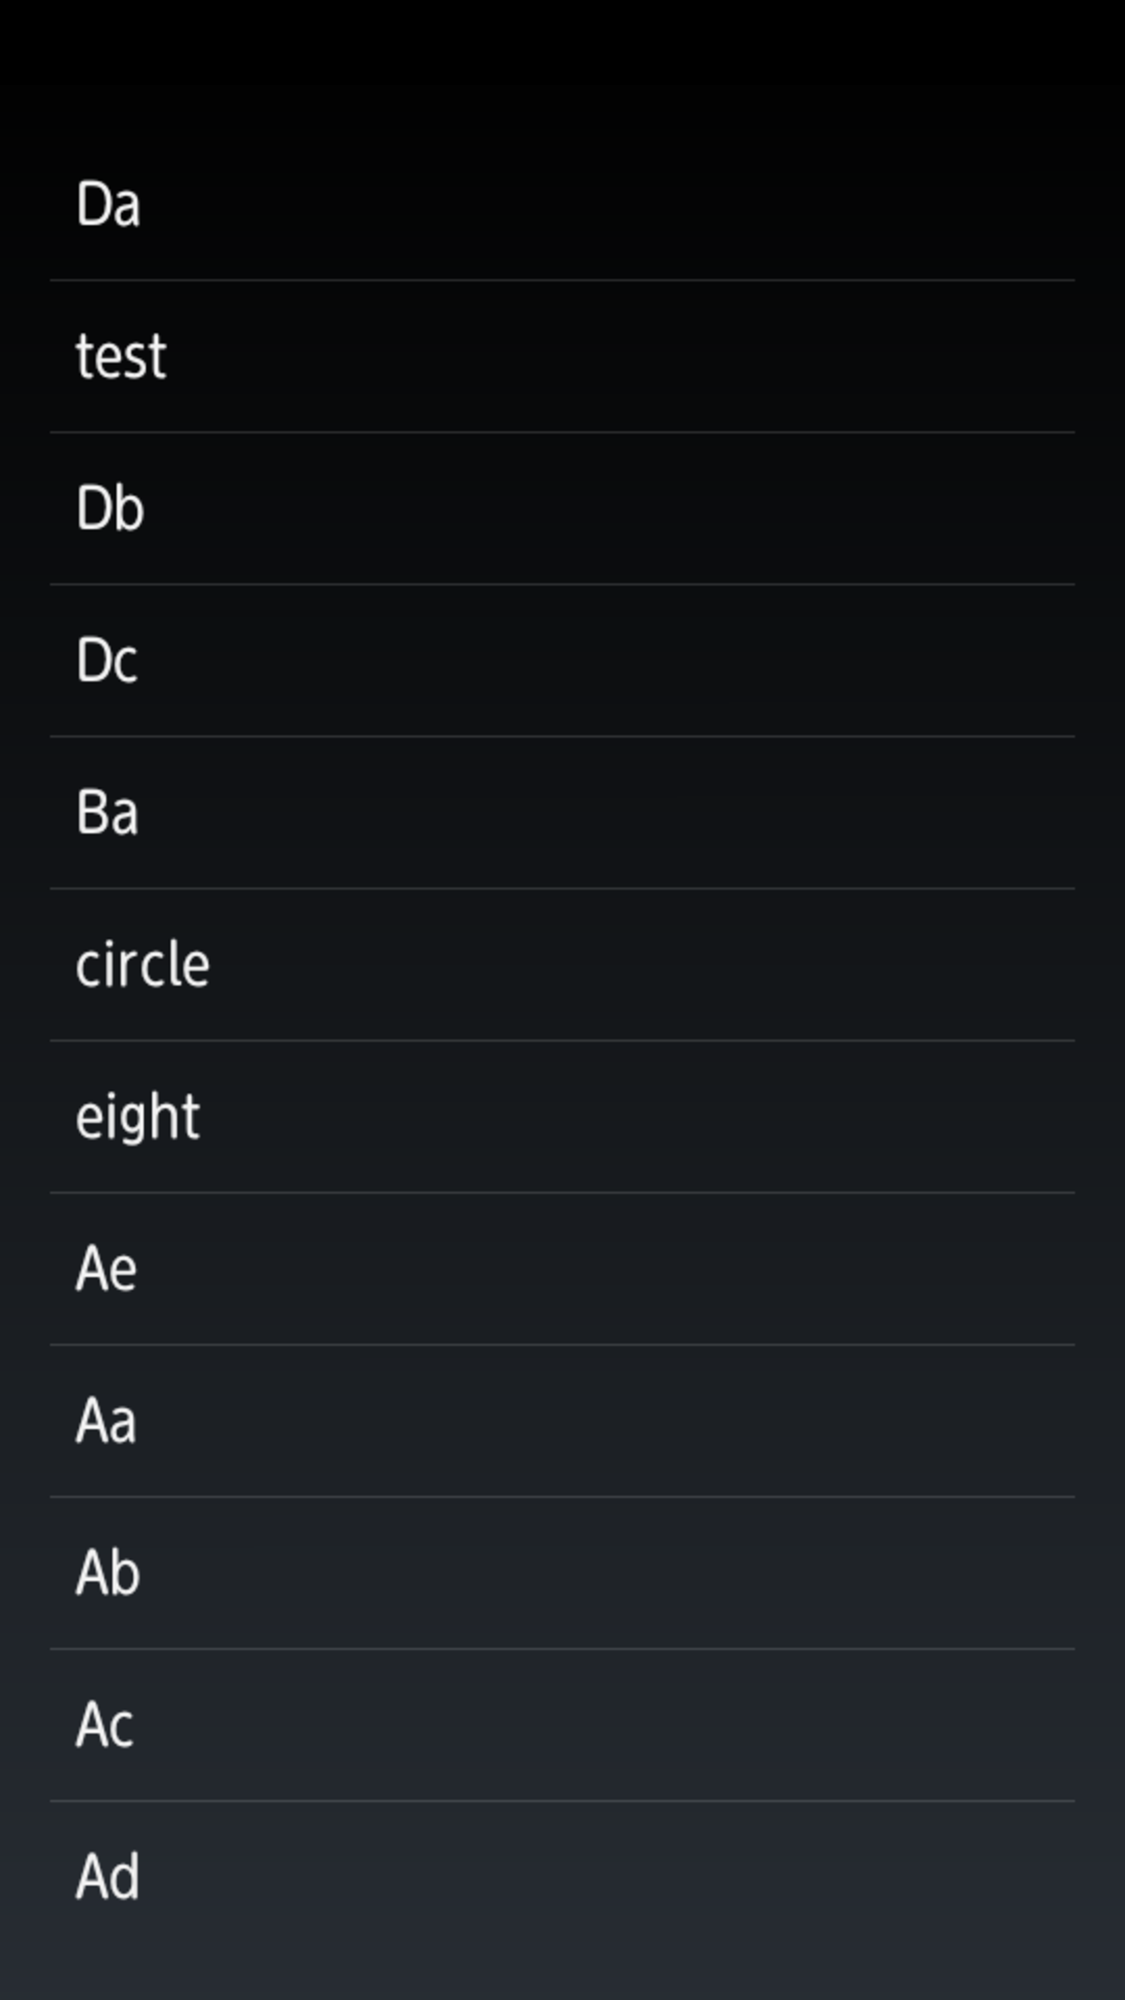
\includegraphics[width=5cm, bb=0 0 540 960]{UserList.pdf}
                \end{center}
                \caption{ユーザ名一覧画面}
                \label{userList}
            \end{minipage}
            \begin{minipage}{0.5\hsize}
                \begin{center}
                    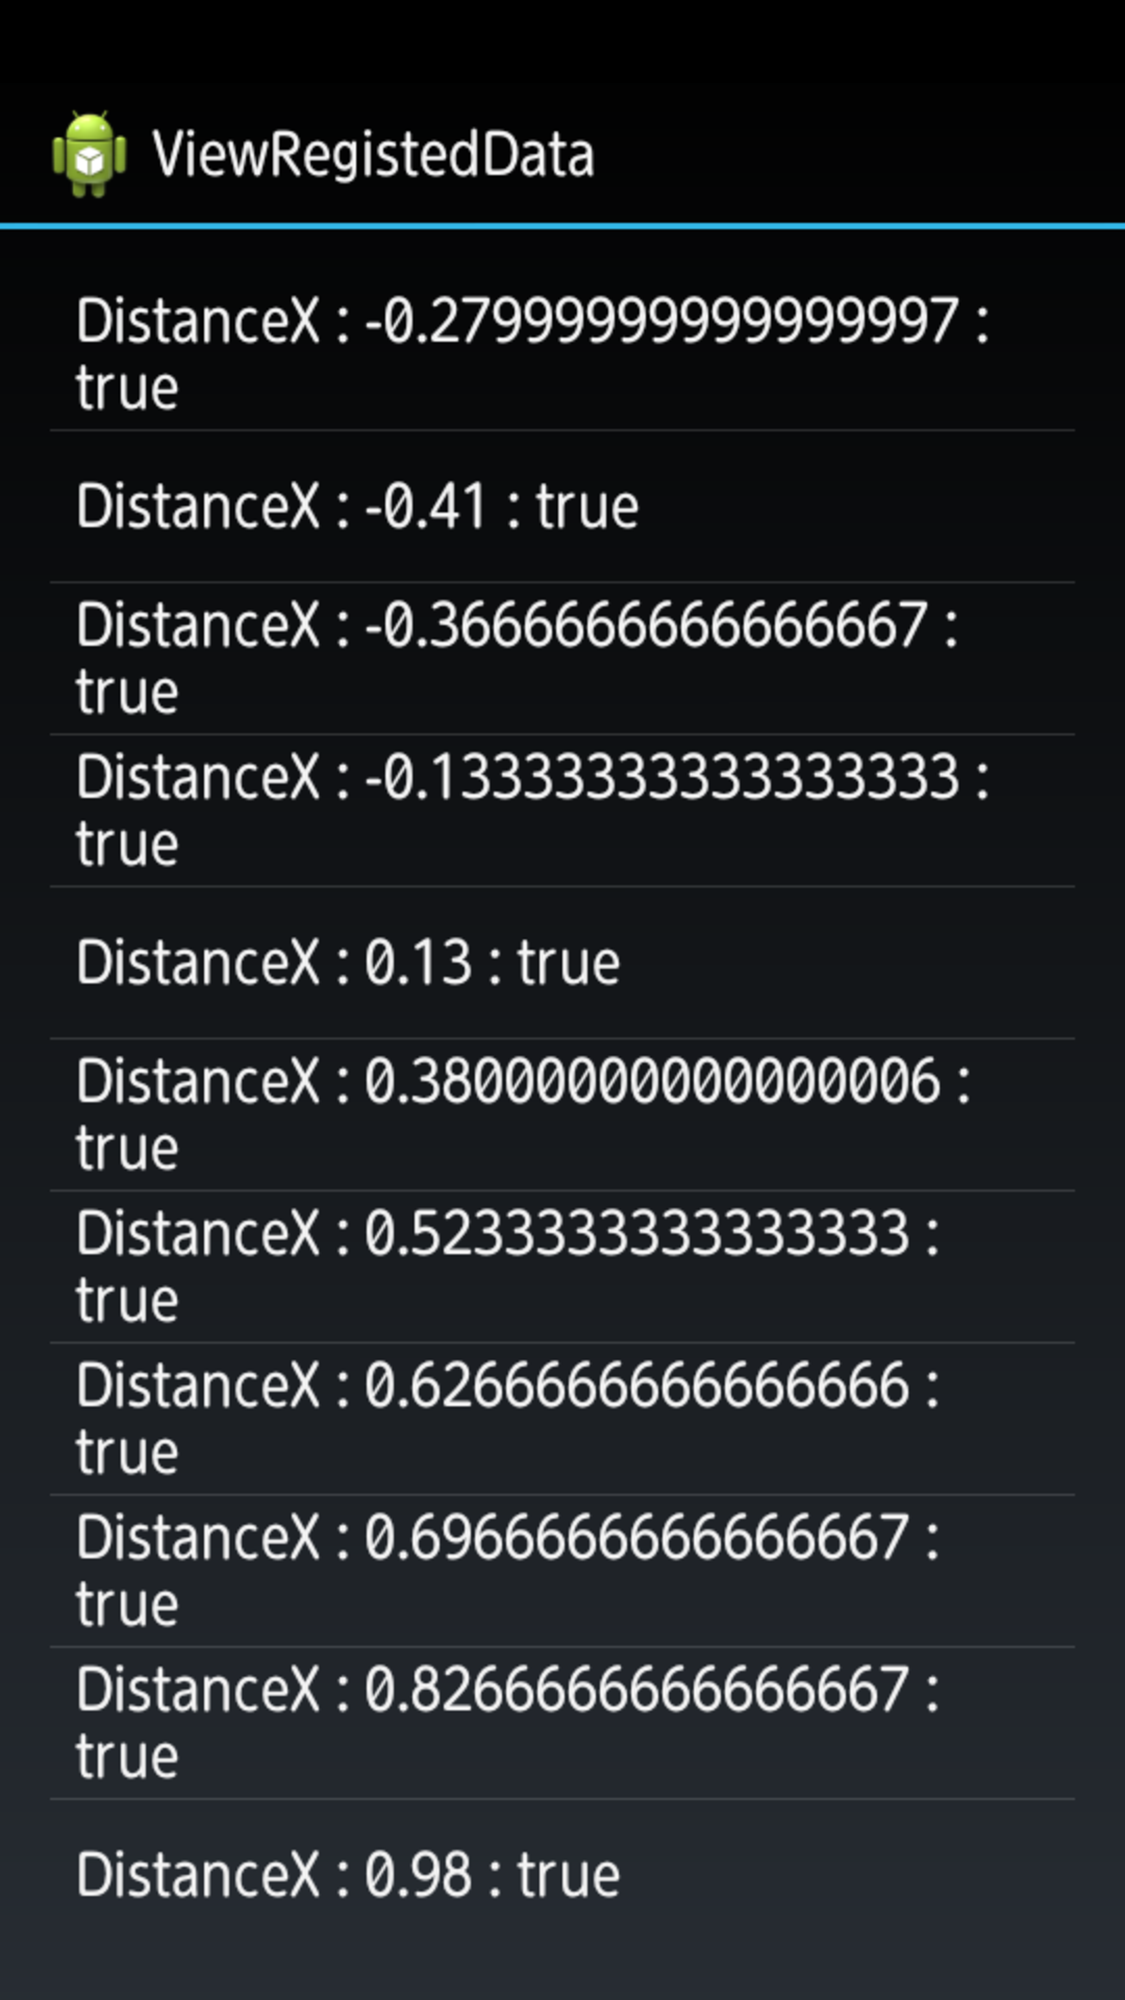
\includegraphics[width=5cm, bb=0 0 540 960]{DataList.pdf}
                \end{center}
                \caption{モーションデータ一覧画面}
                \label{dataList}
            \end{minipage}
        \end{figure}

    \section{先行研究からの改善点}
    先行研究において指摘されていた,手首のスナップを用いるような比較的動きの小さなモーションにおいて,認証率が低く出てしまうという課題を解決するために導入した機能をここに挙げる.

        \subsection{モーション取得時のズレを修正する機能}
        新規登録モードにおいてモーションを登録する際,三回分のモーションデータの入力が必要になるが,この回数ごとにモーションの時間的なズレが生じた場合,データ登録や認証時に影響を与えてしまう可能性があるため,このズレを修正する処理を三回分のデータ取得後に行うようにしている.

        三回分のデータ取得後,まずはこのデータ間の相関係数を算出し,回数ごとに全く別のモーションが入力されていないかの確認を行う.
        そしてある程度以上の相関が見られるが,それでも相関係数が低く出てしまった場合に,ズレ修正後の相関係数を確認しつつ,データの最大値に合わせるパターン,データの最小値に合わせるパターン,データの中央値に合わせるパターンの最大3つの方法で相関係数の向上を試みる.
        この部分をソースコード\ref{checkDeviation}に示す.

        \begin{lstlisting}[caption=ズレ修正前の相関係数チェック, label=checkDeviation]
// measureCorrelation用の平均値データを作成
for (int i = 0; i < 3; i++) {
    for (int j = 0; j < 100; j++) {
        averageDistance[i][j] = (distance[0][i][j] + distance[1][i][j] + distance[2][i][j]) / 3;
        averageAngle[i][j] = (angle[0][i][j] + angle[1][i][j] + angle[2][i][j]) / 3;
    }
}

//region 同一のモーションであるかの確認をし,必要に応じてズレ修正を行う
Enum.MEASURE measure = mCorrelation.measureCorrelation(distance, angle, averageDistance, averageAngle);

LogUtil.log(Log.DEBUG, "After measure correlation");
LogUtil.log(Log.DEBUG, "measure = " + String.valueOf(measure));


if (Enum.MEASURE.BAD == measure) {
    // 相関係数が0.4以下
    return false;
}
else if (Enum.MEASURE.INCORRECT == measure) {
    // 相関係数が0.4よりも高く,0.6以下の場合
    // ズレ修正を行う
    int time = 0;
    Enum.MODE mode = Enum.MODE.MAX;

    double[][][] originalDistance = distance;
    double[][][] originalAngle = angle;

    while (true) {
        switch (time) {
            case 0:
                mode = Enum.MODE.MAX;
                break;
            case 1:
                mode = Enum.MODE.MIN;
                break;
            case 2:
                mode = Enum.MODE.MEDIAN;
                break;
        }

        distance = mCorrectDeviation.correctDeviation(originalDistance, mode);
        angle = mCorrectDeviation.correctDeviation(originalAngle, mode);

        for (int i = 0; i < 3; i++) {
            for (int j = 0; j < 100; j++) {
                averageDistance[i][j] = (distance[0][i][j] + distance[1][i][j] + distance[2][i][j]) / 3;
                averageAngle[i][j] = (angle[0][i][j] + angle[1][i][j] + angle[2][i][j]) / 3;
            }
        }

        Enum.MEASURE tmp = mCorrelation.measureCorrelation(distance, angle, averageDistance, averageAngle);

        if (tmp == Enum.MEASURE.PERFECT || tmp == Enum.MEASURE.CORRECT) {
            break;
        }
        else if (time == 2) {
            // 相関係数が低いまま,アラートなどを出す?
            distance = originalDistance;
            angle = originalAngle;
            break;
        }

        time++;
    }
}
else if (Enum.MEASURE.PERFECT == measure || Enum.MEASURE.CORRECT == measure) {
    // PERFECTなら,何もしない
}
else {
    // なにかがおかしい
    return false;
}
        \end{lstlisting}
        
        相関係数を算出した結果,ズレ修正が必要であると判断された場合,ソースコード\ref{correctDeviation}を用いて修正を行う.

        \begin{lstlisting}[caption=ズレ修正アルゴリズム, label=correctDeviation]
public class CorrectDeviation {

    /**
     * 取得回数ごとのデータのズレを時間的なズレを修正する
     *
     * @param data 修正するdouble型の3次元配列データ
     * @return newData ズレ修正後のdouble型の3次元配列データ
     */
    public double[][][] correctDeviation (double[][][] data, Enum.MODE mode) {
        LogUtil.log(Log.INFO);

        double[][][] newData = new double[3][3][100];

        // 試行回ごとの代表値の出ている時間を抽出
        // 変数は.桁揃え,計算後のdistance, angleを利用

        // 回数・XYZを配列で
        double value[][] = new double[3][3];

        // 代表値の出ている時間,回数,XYZ
        int count[][] = new int[3][3];

        // とりあえず,変数にXYZそれぞれの一個目の値を放り込む
        for (int i = 0; i < 3; i++) {
            for (int j = 0; j < 3; j++) {
                value[i][j] = data[i][j][0];
            }
        }


        // 代表値が出ている場所を取得する
        switch (mode) {
            case MAX:
                for (int i = 0; i < 3; i++) {
                    for (int j = 0; j < 3; j++) {
                        for (int k = 0; k < 100; k++) {
                            if (value[i][j] < data[i][j][k]) {
                                value[i][j] = data[i][j][k];
                                count[i][j] = k;
                            }
                        }
                    }
                }
                break;
            case MIN:
                for (int i = 0; i < 3; i++) {
                    for (int j = 0; j < 3; j++) {
                        for (int k = 0; k < 100; k++) {
                            if (value[i][j] > data[i][j][k]) {
                                value[i][j] = data[i][j][k];
                                count[i][j] = k;
                            }
                        }
                    }
                }
                break;
            case MEDIAN:
                // キーが自動ソートされるTreeMapを用いる.データと順番を紐付けしたものを作成し,中央値の初期の順番の値を取り出す.
                for (int i = 0; i < 3; i++) {
                    for (int j = 0; j < 3; j++) {
                        TreeMap<Double, Integer> treeMap = new TreeMap<>();

                        for (int k = 0; k < 100; k++) {
                            treeMap.put(data[i][j][k], k);
                        }

                        int loopCount = 0;
                        for (Integer initCount : treeMap.values()) {
                            if (loopCount == 49) {
                                count[i][j] = initCount;
                            }

                            loopCount++;
                        }
                    }
                }
                break;
        }
        // 1回目のデータの代表値が出た場所と,2回目・3回目のデータの代表値が出た場所の差をとる
        // とったら,その差だけデータをずらす(ずらしてはみ出たデータは空いたとこに入れる)

        // sample
        // 一回目:50,二回目:30 → 右に20ずらす 一回目-二回目=+20
        // 一回目:30,二回目:50 → 左に20ずらす 一回目-二回目=-20

        // ずらす移動量を計算(XYZそれぞれ)
        int lagData[][] = new int[2][3];


        ArrayList<ArrayList<ArrayList<Double>>> tmpData = new ArrayList<>();

        ArrayList<ArrayList<Double>> tmpData1 = new ArrayList<>();
        ArrayList<Double> tmpData1X = new ArrayList<>();
        ArrayList<Double> tmpData1Y = new ArrayList<>();
        ArrayList<Double> tmpData1Z = new ArrayList<>();

        tmpData1.add(tmpData1X);
        tmpData1.add(tmpData1Y);
        tmpData1.add(tmpData1Z);

        ArrayList<ArrayList<Double>> tmpData2 = new ArrayList<>();
        ArrayList<Double> tmpData2X = new ArrayList<>();
        ArrayList<Double> tmpData2Y = new ArrayList<>();
        ArrayList<Double> tmpData2Z = new ArrayList<>();

        tmpData2.add(tmpData2X);
        tmpData2.add(tmpData2Y);
        tmpData2.add(tmpData2Z);

        tmpData.add(tmpData1);
        tmpData.add(tmpData2);

        for (int i = 0; i < 2; i++) {
            for (int j = 0; j < 3; j++) {
                for (int k = 0; k < 100; k++) {
                    tmpData.get(i).get(j).add(data[i][j][k]);
                }
            }
        }


        // どれだけズレているかを計算する
        for (int i = 0; i < 3; i++) {
            lagData[0][i] = count[0][i] - count[1][i];
            LogUtil.log(Log.DEBUG, "lagData[0]" + "[" + i + "]" + ": " + lagData[0][i]);

            lagData[1][i] = count[0][i] - count[2][i];
            LogUtil.log(Log.DEBUG, "lagData[1]" + "[" + i + "]" + ": " + lagData[1][i]);
        }


        // 実際にリストの要素をずらしていく

        for (int i = 0; i < 2; i++) {
            for (int j = 0; j < 3; j++) {
                Collections.rotate(tmpData.get(i).get(j), lagData[i][j]);
            }
        }


        // これでずらせたはずだ.成果はリストに入っているはずなので,ずらした後のデータを専用の配列に入れよう
        // 1回目のデータに関しては基準となるデータなのでそのまま入れる
        for (int i = 0; i < 3; i++) {
            for (int j = 0; j < 100; j++) {
                newData[0][i][j] = data[0][i][j];
            }
        }

        // ずらしたデータを入れる
        for (int i = 0; i < 2; i++) {
            for (int j = 0; j < 3; j++) {
                for (int k = 0; k < 100; k++) {
                    newData[i + 1][j][k] = tmpData.get(i).get(j).get(k);
                }
            }
        }

        return newData;
    }
}
        \end{lstlisting}

        \subsection{フーリエ変換を用いたローパスフィルタ}
        モーションデータを取得している際の,細かな手の震えなどによるデータに対する影響を取り除き,モーションデータとしての純度を高めるために,フーリエ変換を用いたローパスフィルタ処理を行っている.

        フーリエ変換を用いて時間軸で表されるモーションデータを周波数領域に変換することで,モーション中の細かな手の震えなどのデータが高周波成分として現れる.
        そしてこの高周波成分を取り除いた上で元の時間軸のデータに戻すローパスフィルタ処理を行うことで,細かな手の震えなどによるデータに対する影響を取り除いている.
        この処理をソースコード\ref{lowpass}に示す.

        \begin{lstlisting}[caption=ローパスフィルタ処理, label=lowpass]
/**
 * double型三次元配列の入力データに対し,フーリエ変換を用いてローパスフィルタリングを行ってデータの平滑化を行う
 *
 * @param data     データ平滑化を行うdouble型三次元配列データ
 * @param dataName アウトプット用,データ種別
 * @return フーリエ変換によるローパスフィルタリングにより滑らかになったdouble型三次元配列データ
 */
public double[][][] LowpassFilter (double[][][] data, String dataName) {
    LogUtil.log(Log.INFO);

    DoubleFFT_1D realfft = new DoubleFFT_1D(data[0][0].length);

    // フーリエ変換(ForwardDFT)の実行
    for (double[][] i : data) {
        for (double[] j : i) {
            realfft.realForward(j);
        }
    }


    // 実数部,虚数部それぞれを入れる配列
    double[][][] real = new double[data.length][data[0].length][data[0][0].length];
    double[][][] imaginary = new double[data.length][data[0].length][data[0][0].length];

    int countReal = 0;
    int countImaginary = 0;

    // 実数部と虚数部に分解
    for (int i = 0; i < data.length; i++) {
        for (int j = 0; j < data[i].length; j++) {
            for (int k = 0; k < data[i][j].length; k++) {
                if (k % 2 == 0) {
                    real[i][j][countReal] = data[i][j][k];
                    countReal++;
                    if (countReal == 99) countReal = 0;
                }
                else {
                    imaginary[i][j][countImaginary] = data[i][j][k];
                    countImaginary++;
                    if (countImaginary == 99) countImaginary = 0;
                }
            }
        }
    }

    mManageData.writeDoubleThreeArrayData("ResultFFT", "rFFT" + dataName, RegistNameInput.name, real);
    mManageData.writeDoubleThreeArrayData("ResultFFT", "iFFT" + dataName, RegistNameInput.name, imaginary);

    // パワースペクトルを求めるために,実数部(k),虚数部(k + 1)それぞれを二乗して加算し,平方根を取り,絶対値を求める
    double[][][] power = new double[data.length][data[0].length][data[0][0].length / 2];

    for (int i = 0; i < data.length; i++) {
        for (int j = 0; j < data[i].length; j++) {
            for (int k = 0; k < data[i][j].length / 2; k++) {
                power[i][j][k] = Math.sqrt(Math.pow(real[i][j][k], 2) + Math.pow(imaginary[i][j][k], 2));
            }
        }
    }

    mManageData.writeDoubleThreeArrayData("ResultFFT", "powerFFT" + dataName, RegistNameInput.name, power);

    // ローパスフィルタ処理
    for (int i = 0; i < data.length; i++) {
        for (int j = 0; j < data[i].length; j++) {
            for (int k = 0; k < data[i][j].length; k++) {
                if (k > 30) data[i][j][k] = 0;
            }
        }
    }

    for (double[][] i : data) {
        for (double[] j : i) {
            realfft.realInverse(j, true);
        }
    }

    mManageData.writeDoubleThreeArrayData("AfterFFT", dataName, RegistNameInput.name, data);

    return data;
}
        \end{lstlisting}

        \subsection{モーションデータの増幅機能}
        手首を中心とするような動きの小さいモーションにおける個人認証成功率を向上させるために,モーションデータの増幅機能を実装した.
        これにより,比較的動きの小さなモーションであってもデータを増幅して用いることができ,比較的動きの大きなモーションと比べて遜色なく用いることが出来るようになった.
        この処理をソースコード\ref{amplifier}に示す.

        \begin{lstlisting}[caption=モーションデータ増幅機能, label=amplifier]
/**
 * 与えられたデータを増幅させる
 *
 * @param data 増幅させるdouble型三次元配列データ
 * @param ampValue どれだけデータを増幅させるか   
 * @return 増幅後のdouble型三次元配列データ
 */
public double[][][] Amplify (double[][][] data, double ampValue) {
    LogUtil.log(Log.INFO);

    if (ampValue != 0.0) {
        for (int i = 0; i < data.length; i++) {
            for (int j = 0; j < data[i].length; j++) {
                for (int k = 0; k < data[i][j].length; k++) {
                    data[i][j][k] *= ampValue;
                }
            }
        }
    }
    return data;
}
        \end{lstlisting}

        この増幅機能は,事前にデータの最大値と最小値の差を取り,得られた値があらかじめ設定された閾値を下回った場合にのみ機能するようにしている.
        この処理をソースコード\ref{dataRangeCheck}に示す.

        \begin{lstlisting}[caption=データレンジチェック, label=dataRangeCheck]
private boolean isRangeCheck = false;


/**
 * 全試行回数中,一回でもデータの幅が閾値よりも小さければtrueを返す
 *
 * @param data チェックするdouble型三次元配列データ
 * @return 全試行回数中,一回でもデータの幅が閾値よりも小さければtrue,そうでなければfalse
 */
public boolean CheckValueRange (double[][][] data, double checkRangeValue) {
    LogUtil.log(Log.INFO);

    LogUtil.log(Log.DEBUG, "checkRangeValue" + checkRangeValue);

    double[][] max = new double[data.length][data[0].length];
    double[][] min = new double[data.length][data[0].length];

    for (int i = 0; i < data.length; i++) {
        for (int j = 0; j < data[i].length; j++) {
            max[i][j] = 0;
            min[i][j] = 0;
        }
    }

    double range;
    for (int i = 0; i < data.length; i++) {
        for (int j = 0; j < data[i].length; j++) {
            for (int k = 0; k < data[i][j].length; k++) {
                if (data[i][j][k] > max[i][j]) {
                    max[i][j] = data[i][j][k];
                }
                else if (data[i][j][k] < min[i][j]) {
                    min[i][j] = data[i][j][k];
                }
            }
        }
    }

    for (int i = 0; i < max.length; i++) {
        for (int j = 0; j < max[i].length; j++) {
            range = max[i][j] - min[i][j];
            LogUtil.log(Log.DEBUG, "range = " + range);
            if (range < checkRangeValue) isRangeCheck = true;
        }
    }

    return isRangeCheck;
}
        \end{lstlisting}

        データをどれだけ増幅させるかを決める値や,データの最大値と最小値の差がどれだけあれば増幅を行うかを決める閾値に関しては,新規登録モードにおいてメニューキーを押すことで表示される,図\ref{regMenu}のようなメニューアイテム内の増幅器設定を選択することで表示される,図\ref{amplifierSettings}のような設定ダイアログより変更することが出来る.

    \begin{figure}[htbp]
        \begin{minipage}{0.5\hsize}
            \begin{center}
                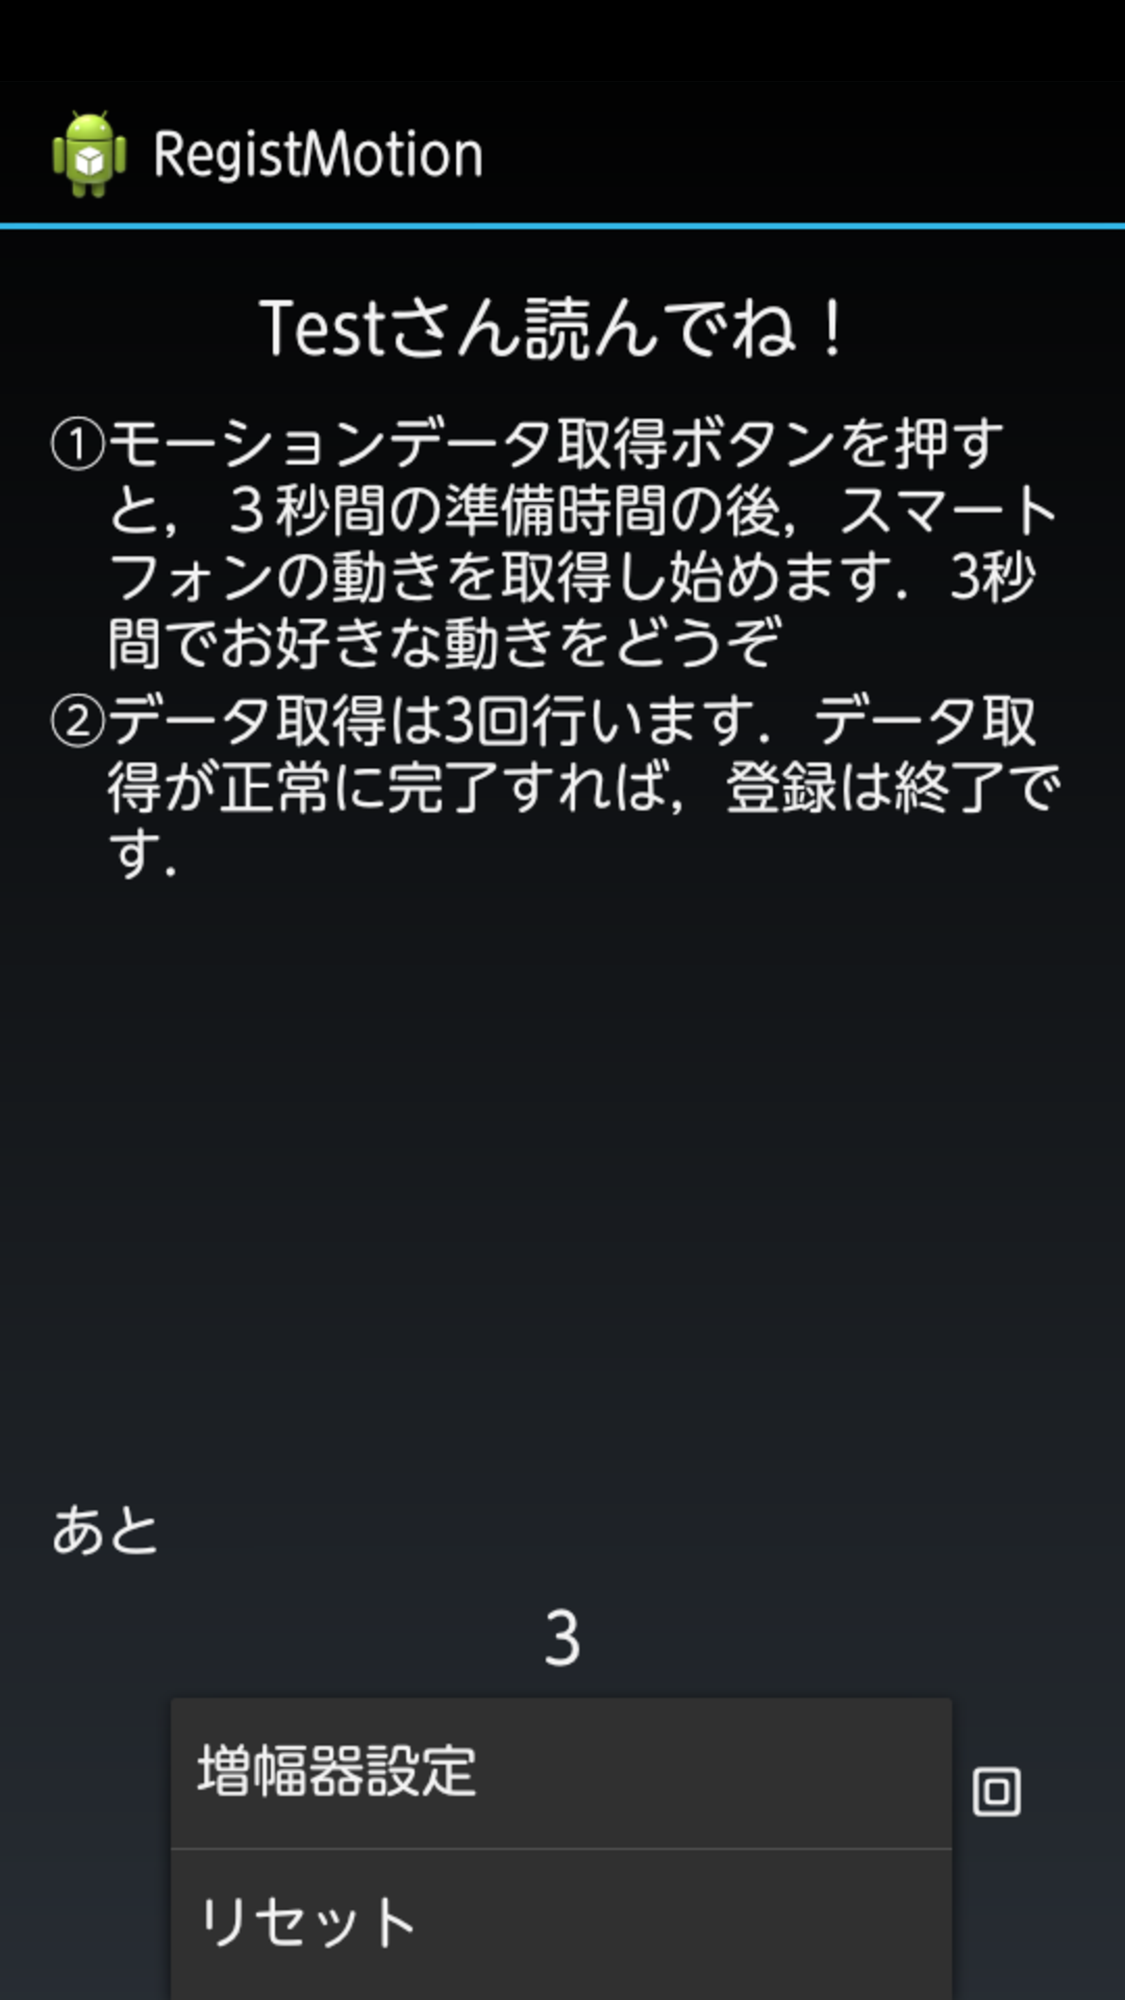
\includegraphics[width=5cm, bb=0 0 540 960]{RegMenu.pdf}
            \end{center}
            \caption{新規登録モードメニュー画面}
            \label{regMenu}
        \end{minipage}
        \begin{minipage}{0.5\hsize}
            \begin{center}
                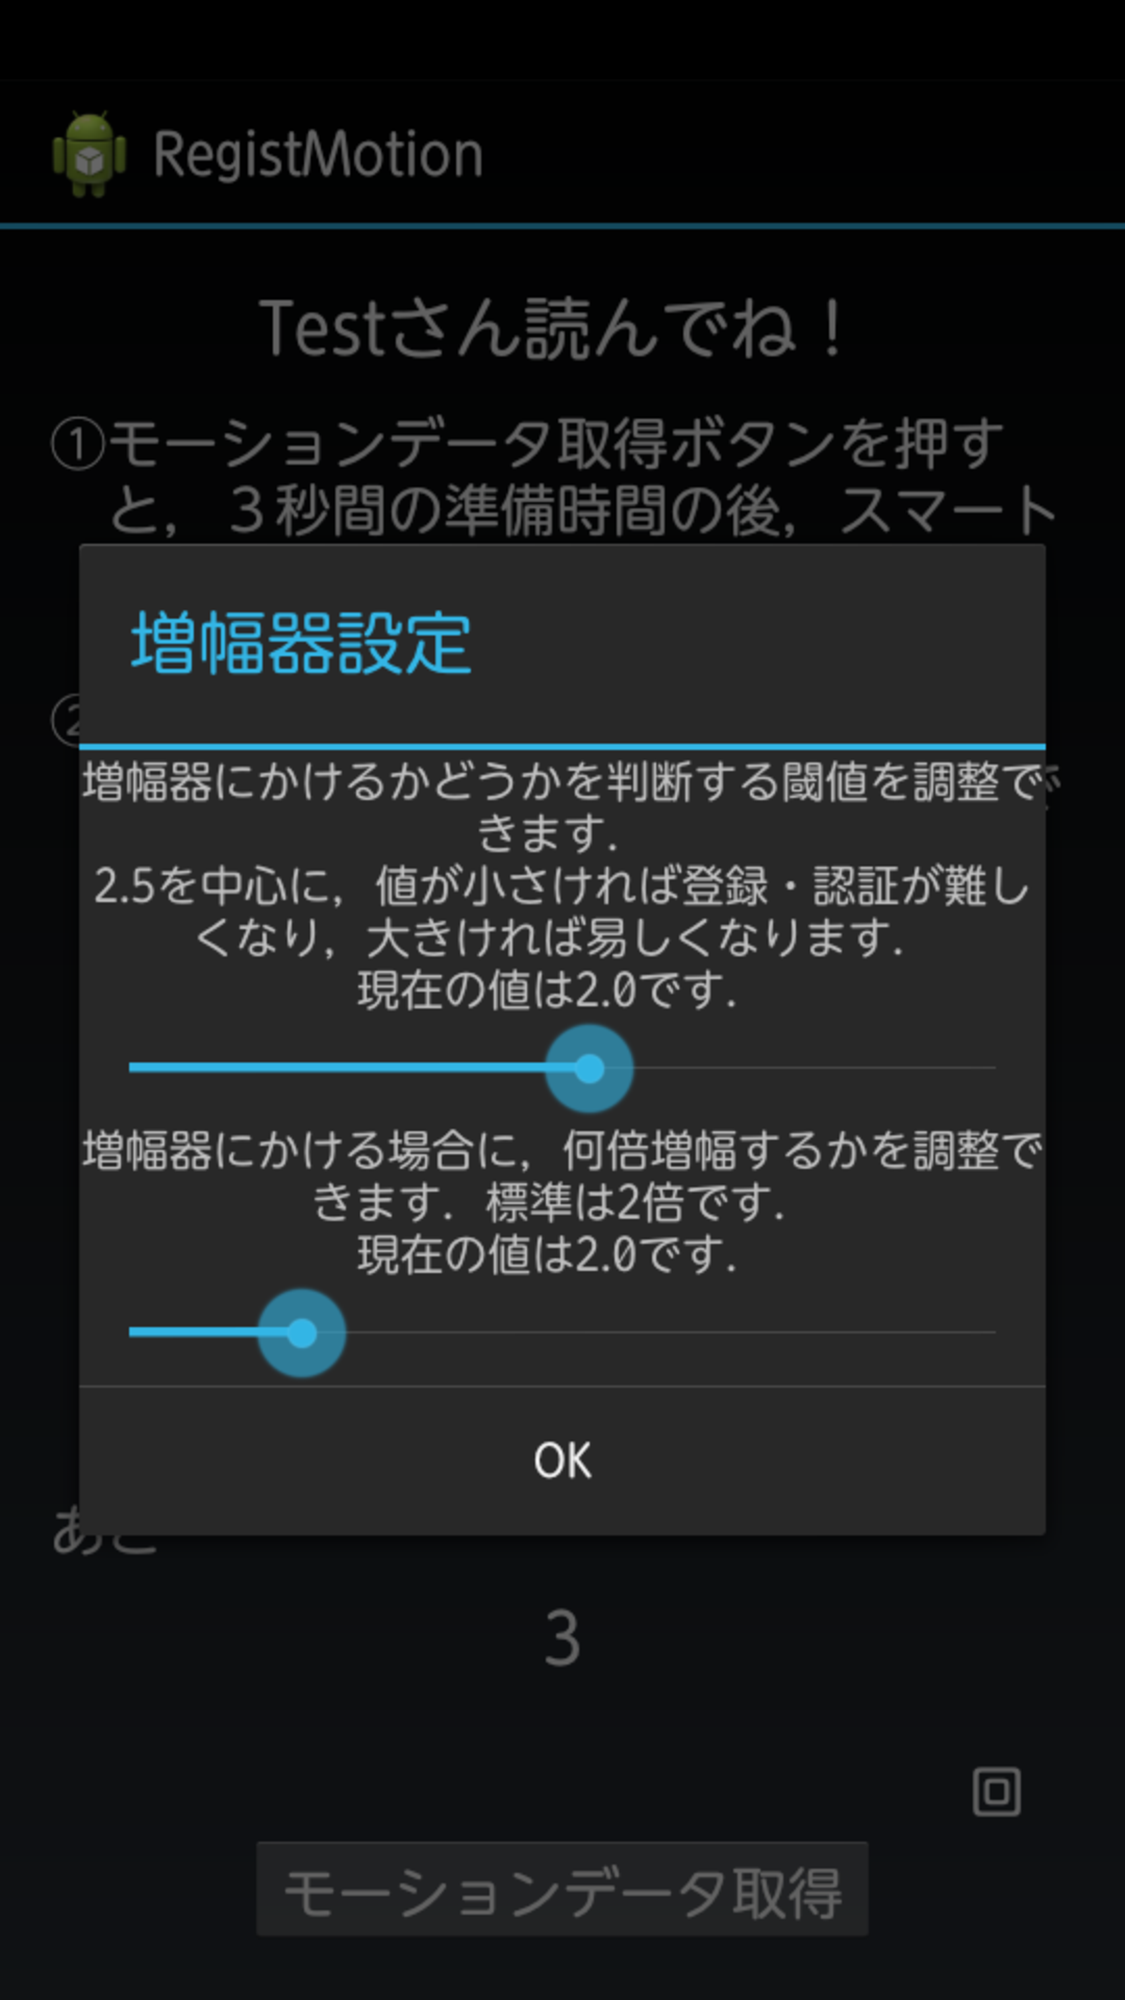
\includegraphics[width=5cm, bb=0 0 540 960]{AmplifierSettings.pdf}
            \end{center}
            \caption{増幅器設定ダイアログ}
            \label{amplifierSettings}
        \end{minipage}
    \end{figure}

        \subsection{モーション取得時のインターバル及びヴァイブレーション機能}
        新規登録モード及び認証試験モードにおいて,モーション取得時の時間経過が把握しやすいように,一秒毎に端末をヴァイブレーションさせる機能を実装した.
        また,データ取得時のインターバルからデータ取得に移る際には通常よ長めのヴァイブレーションにすることで,データ取得開始のタイミングを明確に意識できるようにした.

\chapter{実験と考察}
	\section{実験方法}
	今回開発したシステムを用いて,以下に挙げるそれぞれのモーションを新規登録モードにてあらかじめ登録しておき,認証試験モードにて個人認証の成功率を検証する.
    認証はそれぞれのモーションにつき十回ずつ行い,この結果から個人認証の成功率を算出する.

	\section{実験結果}
	\textcolor{red}{実験結果を表を用いて示す}

	\section{考察}
    \textcolor{red}{実験結果に対する考察}

	\section{課題}
	\textcolor{red}{実験結果より生じた課題}

\chapter{おわりに}

\chapter*{謝辞}
本研究のプログラム開発や実験,本論文の執筆にあたり,手厚い指導と様々な助言をしていただいた,関西大学総合情報学部セキュア情報システム研究室の小林孝史准教授に深く感謝いたします.
また,研究テーマの選定をはじめ,日頃から有益なアドバイスを頂いた同研究室の皆様に感謝いたします.

\end{document}
